%!TEX root = ../template.tex
%%%%%%%%%%%%%%%%%%%%%%%%%%%%%%%%%%%%%%%%%%%%%%%%%%%%%%%%%%%%%%%%%%%%
%% F2_stateoftheart.tex
%% NOVA thesis document file
%%
%% Chapter with lots of dummy text
%%%%%%%%%%%%%%%%%%%%%%%%%%%%%%%%%%%%%%%%%%%%%%%%%%%%%%%%%%%%%%%%%%%%

\typeout{NT FILE F2_stateoftheart.tex}%


%%%%%%%%%%%%%%%%%%%%%%%%%%%%%%%%%%%%%%%%%%%%%%%%%%
\chapter{Estado da Arte}
\label{cha:estado_da_arte}
%%%%%%%%%%%%%%%%%%%%%%%%%%%%%%%%%%%%%%%%%%%%%%%%%%

\section{Redes Veiculares}
\label{sec:redes_veic}
%%%%%%%%%%%%%%%%%%%%%%%%%%%%%%%%%%%%%%%%%%%%%%%%%%

As redes ad-hoc veiculares (VANETs) constituem uma variante especial das redes móveis ad-hoc \gls{MANETs} onde os veículos atuam como nós móveis da rede comunicando entre si e com
a infraestrutura da rede \cite{khelifi_named_2020}. No contexto das \gls{VANETs} incluem-se diferentes modos de comunicação, tais como \gls{V2V}, \gls{V2I}, \gls{V2P}, \gls{V2N} e \gls{V2X}, conforme ilustrado na Figura~\ref{fig:V2X}. Além disso, estes modos integram o paradigma cooperativo de transporte inteligente, no qual a troca contínua de mensagens suporta funcionalidades avançadas de segurança e automação.

\begin{figure}[h]
    \centering
    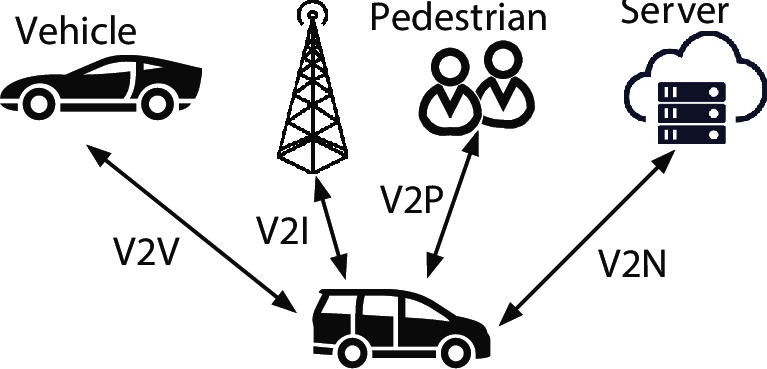
\includegraphics[width=0.5\textwidth]{Chapters/Figures/V2X.png}
    \caption{Mensagens das \gls{VANETs} \cite{noauthor_figure_nodate}}
    \label{fig:V2X}
\end{figure}

\subsection{Arquitetura e Componentes (OBU–RSU)}
\label{sec:arquitetura}

A arquitetura das \gls{VANETs} assenta em dois componentes principais: as unidades nos veículos (\gls{OBUs}) e as unidades fixas na infraestrutura rodoviária (\gls{RSUs}).

As \textbf{\gls{OBUs}} estão instaladas nos veículos, tipicamente no interior do habitáculo ou integradas na unidade telemática do veículo. São responsáveis por processar informação sensorial local, armazenar dados temporariamente e comunicar com outros veículos ou com a infraestrutura. Incluem normalmente módulos de posicionamento, processadores de bordo e interfaces rádio compatíveis com IEEE 802.11p ou C-V2X. Para além disso, as OBUs agregam sensores e atuadores do veículo, permitindo a integração com sistemas avançados de assistência à condução.

As \textbf{\gls{RSUs}} são dispositivos fixos montados em elementos da via, como semáforos, postes de iluminação, portagens, cruzamentos ou entradas de autoestradas. Estão estrategicamente posicionadas para maximizar a cobertura e garantir visibilidade direta dos veículos. Atuando como pontos de acesso distribuídos, estendem a conectividade da rede e permitem a ligação aos sistemas centrais de gestão de tráfego. Em muitos cenários, as RSUs suportam também computação de borda, permitindo processar dados localmente e reduzir a latência de aplicações críticas.

Esta arquitetura, definida em normas como o \textit{ETSI ITS-G5} e o \textit{3GPP C-V2X}, fornece a base para aplicações cooperativas que exigem baixas latências, elevada fiabilidade e comunicação persistente em cenários complexos \cite{gerla_internet_2014}.

\subsection{Tecnologias de Comunicação V2X}
\label{sec:tecnologias_v2x}

Os modos \gls{V2V} e \gls{V2I} utilizam sobretudo duas tecnologias padrão: \textbf{IEEE 802.11p (ITS-G5)} e \textbf{C-V2X}, definidas respetivamente pelo \textit{IEEE/ETSI} e pelo \textit{3GPP}. Ambas suportam comunicação direta, mas diferem nos mecanismos físicos e no desempenho.

\paragraph{IEEE 802.11p (ITS-G5).}  
Permite comunicação direta de curto alcance com latências reduzidas (da ordem dos milissegundos), mas é sensível à congestão do canal em cenários de elevada densidade, devido ao mecanismo de contenção do meio. É amplamente utilizado na norma europeia \textit{ETSI ITS-G5}. Em ambientes densos pode ocorrer o fenómeno de \textit{broadcast storm}, onde transmissões simultâneas causam colisões e perda de desempenho.

\paragraph{C-V2X (3GPP).}  
Opera em modo direto (\textit{sidelink} PC5) e em modo assistido pela rede. Utiliza programação sem necessidade de contenção, o que reduz colisões e melhora a fiabilidade em cenários densos. Nas evoluções 5G (NR-V2X), oferece maior alcance, mais robustez e suporte nativo a baixa latência. Este modo introduz ainda melhor suporte para condução cooperativa e aplicações de automação avançada.

\paragraph{Comparação técnica resumida.}
\begin{itemize}
    \item \textit{Acesso ao meio:} 802.11p usa contenção (mais colisões em ambientes densos); C-V2X utiliza agendamento semi-persistente (melhor fiabilidade).
    \item \textit{Alcance:} 802.11p é tipicamente limitado a 300-500 m; C-V2X pode atingir 1 km em modo PC5.
    \item \textit{Latência:} ambos suportam latências baixas, mas C-V2X mantém-nas de forma mais estável sob carga elevada.
    \item \textit{Interoperabilidade futura:} 5G NR-V2X expande capacidades para condução cooperativa e veículos autónomos, enquanto 802.11p apresenta limitações para evoluções mais complexas.
\end{itemize}

A disseminação das mensagens é feita por \textit{broadcast} ou \textit{geocast} no caso de \gls{V2V}, enquanto na \gls{V2I} as \gls{RSUs} reencaminham dados para sistemas centrais, permitindo coordenação global.

\subsection{Aplicações}
\label{sec:aplicacoes}

As \gls{VANETs} suportam três grandes categorias de aplicações: de segurança, de gestão de tráfego e de
conforto \textit{(infotainment)}, conforme ilustrado (Figura~\ref{fig:apps}), cada uma com requisitos distintos de latência, fiabilidade e largura de banda . Estas aplicações cooperativas utilizam mensagens padronizadas como CAM e DENM, fundamentais para a operação segura dos sistemas ITS europeus.

\begin{figure}[h]
    \centering
    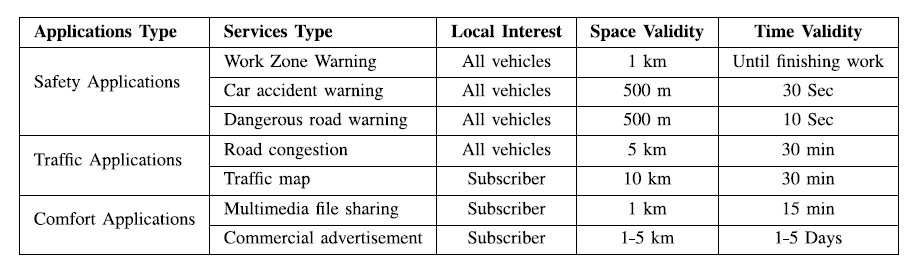
\includegraphics{Chapters/Figures/VANETs_apps.png}
    \caption{Aplicações das \gls{VANETs} \cite{khelifi_named_2020}}
    \label{fig:apps}
\end{figure}

\paragraph{Aplicações de segurança.}  
visam reduzir acidentes e aumentar a segurança rodoviária, através
da disseminação de mensagens críticas, como alertas de colisão, travagem de emergência, ou
deteção de veículos em ângulo morto. Estas aplicações exigem latência extremamente baixa (da
ordem dos milissegundos) e elevada fiabilidade \cite{al-ani_survey_2018}. São reguladas por normas como ETSI ITS-G5 CAM/DENM.

\paragraph{Aplicações de gestão de tráfego.}  
permitem otimizar fluxos rodoviários, reduzindo congestionamentos
e tempos de viagem. Exemplos incluem coordenação de semáforos inteligentes e partilha
de informações sobre condições da via ou obras. As exigências de latência são moderadas, mas requerem cobertura ampla via \gls{V2I} \cite{jayapal_road_2016}.

\paragraph{Aplicações de conforto}  
fornecem serviços não críticos, como streaming, acesso à internet,
atualização de mapas ou comunicações sociais entre veículos. Estas aplicações toleram maiores
latências, mas requerem maior largura de banda e mecanismos eficientes de disseminação de
conteúdo., sendo frequentemente suportadas por \gls{V2N} ou redes celulares.

\subsection{Desafios Técnicos das VANETs}
\label{sec:desafios}

Apesar dos avanços tecnológicos, as \gls{VANETs} enfrentam desafios significativos: \begin{itemize} \item \textbf{Escalabilidade:} Em cenários urbanos com elevada densidade de veículos, o número de mensagens de controlo e retransmissões pode crescer exponencialmente, levando à congestão do canal e degradação de desempenho. O \gls{MAC} e o encaminhamento eficiente são essenciais para manter a escalabilidade. \item \textbf{Mobilidade elevada e topologia dinâmica:} A rápida variação da vizinhança entre veículos causa quebras de ligação frequentes, dificultando o estabelecimento de rotas persistentes e a disseminação contínua de dados. \item \textbf{Latência e fiabilidade:} As aplicações de segurança exigem comunicações quase instantâneas e altamente fiáveis. A variação do atraso (\textit{jitter}) e as perdas de pacotes podem comprometer a eficácia de mensagens críticas. \item \textbf{Conectividade intermitente:} Em regiões rurais ou com baixa densidade de veículos, as comunicações podem depender de oportunidades de contacto (\textit{store-carry-forward}), exigindo protocolos tolerantes a atrasos e interrupções temporárias. \item \textbf{Segurança e privacidade:} As VANETs são vulneráveis a ataques como \textit{spoofing}, \textit{Sybil} ou \textit{Denial of Service}. A autenticação e a integridade das mensagens são cruciais, mas devem ser implementadas sem comprometer a latência. \item \textbf{Heterogeneidade tecnológica:} A coexistência de diferentes tecnologias (IEEE 802.11p, C-V2X, 5G) impõe desafios de interoperabilidade e coordenação de múltiplos canais de comunicação. \item \textbf{Broadcast storm:} Em cenários densos, a disseminação massiva de mensagens pode provocar redundância e colisões, exigindo técnicas de supressão e temporização. \end{itemize}

Em síntese, as redes veiculares representam um domínio altamente dinâmico e complexo, no qual
a eficiência da comunicação depende da capacidade dos protocolos em lidar com a escalabilidade, mobilidade
e diversidade tecnológica. O paradigma V2X evolui progressivamente para suportar sistemas
cooperativos de transporte inteligente e veículos autónomos, nos quais a comunicação fiável e de baixa
latência é um requisito fundamental para a segurança e o desempenho global da rede \cite{halim_research_2023}.


%%%%%%%%%%%%%%%%%%%%%%%%%%%%%%%%%%%%%%%%%%%%%%%%%%
\section{Redes \gls{NDN}}
\label{sec:redes_NDN}
%%%%%%%%%%%%%%%%%%%%%%%%%%%%%%%%%%%%%%%%%%%%%%%%%%

No início do desenvolvimento da Internet, o modelo de comunicação proposto pelo TCP/IP representou uma solução inovadora para a troca de informações ponto a ponto entre entidades identificadas por endereços. Embora o paradigma IP tenha sido concebido para conversas diretas entre hosts, o seu sucesso levou à sua adoção também em sistemas de distribuição de conteúdos, transformando a Internet numa vasta rede de disseminação de dados. Contudo, esta adaptação revelou limitações: o IP identifica apenas os pontos finais de comunicação, não os próprios conteúdos, tornando a distribuição de informação um processo complexo e ineficiente.

O \gls{NDN} surge como uma evolução arquitetural que visa superar essas limitações, generalizando o modelo da Internet para tornar o conteúdo, e não a localização, o elemento central da comunicação \cite{khelifi_named_2020}. Em vez de endereçar pacotes a um destino específico, o \GLS{NDN} utiliza nomes hierárquicos para identificar diretamente os dados. Essa alteração aparentemente simples introduz uma mudança profunda: a comunicação passa a ser orientada por dados, em que os consumidores expressam interesse pelo conteúdo desejado, e a rede encarrega-se de encontrá-lo e entregá-lo.

A comunicação no NDN envolve dois papéis fundamentais, aqui introduzidos formalmente:
\begin{itemize}
    \item \textbf{Consumidor}: a entidade que expressa um pedido por dados, enviando um pacote \textit{Interest};
    \item \textbf{Produtor}: a entidade que origina ou detém o conteúdo solicitado e responde com um pacote \textit{Data}.
\end{itemize}

A comunicação no \gls{NDN} é conduzida por dois tipos de pacotes: \textit{Interest} e \textit{Data} (Figura~\ref{fig:Packets}). O consumidor envia um pacote de interesse contendo o nome do dado desejado; os routers utilizam esse nome para encaminhar o pedido até um produtor que possua o conteúdo. Quando o interesse atinge um nó que contém os dados, é gerado um pacote de dados, contendo o nome e o conteúdo solicitado, que regressa pelo caminho inverso percorrido pelo interesse.

\begin{figure}[h]
\centering
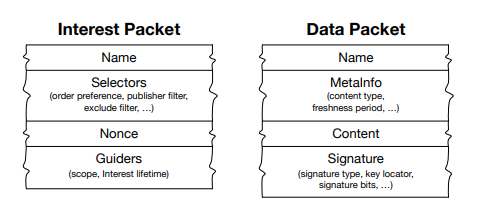
\includegraphics[width=0.75\linewidth]{Chapters/Figures/Packets.png}
\caption{Estrutura básica dos pacotes \gls{NDN} \cite{papadopoulos_lixia_2014}.}
\label{fig:Packets_NDN}
\end{figure}

%%%%%%%%%%%%%%%%%%%%%%%%%%%%%%%%%%%%%%%%%%%%%%%%%%
\subsection{Modelo de comunicação centrado em dados}
\label{sub:NDN_modelo}
%%%%%%%%%%%%%%%%%%%%%%%%%%%%%%%%%%%%%%%%%%%%%%%%%%

No \gls{NDN}, o fluxo de Interest e Data ocorre como se segue:

\begin{enumerate}
    \item O consumidor envia um \textit{Interest} contendo o \textbf{nome do conteúdo} desejado.
    \item A rede encaminha o \textit{Interest} com base em nomes, de forma hop-by-hop.
    \item Quando um nó (router ou produtor) possui o conteúdo, gera um pacote \textit{Data}.
    \item O \textit{Data} regressa ao consumidor seguindo exatamente o caminho inverso do \textit{Interest}, utilizando a informação guardada ao longo do percurso.
\end{enumerate}

Esta comunicação não requer sessões persistentes, endereços IP ou manutenção explícita de rotas fim-a-fim.  


%%%%%%%%%%%%%%%%%%%%%%%%%%%%%%%%%%%%%%%%%%%%%%%%%%
\subsection{Estruturas internas: FIB, PIT e Content Store}
\label{sub:NDN_estruturas}
%%%%%%%%%%%%%%%%%%%%%%%%%%%%%%%%%%%%%%%%%%%%%%%%%%

Para suportar este modelo orientado a dados, cada router NDN mantém três estruturas fundamentais: a \gls{FIB}, a \gls{PIT} e a \gls{CS}. Juntas, estas estruturas permitem à rede encaminhar, armazenar e entregar conteúdos de forma eficiente, sem dependência de endereços IP ou de sessões persistentes. A interação entre estas três tabelas é frequentemente designada por \textit{triângulo de encaminhamento} do \gls{NDN}.

\subsubsection{\gls{CS}}

A \gls{CS} funciona como uma memória \textit{cache} local que armazena temporariamente pacotes de dados previamente recebidos. Quando chega um pacote de interesse, o router verifica primeiro se o conteúdo correspondente já está armazenado na CS. Caso esteja, os dados são devolvidos de imediato pela interface de onde veio o pedido, sem necessidade de contactar o produtor original, caso contrário, prossegue-se para as restantes estruturas. Este mecanismo de \textit{in-network caching} é essencial para reduzir a latência e o consumo de largura de banda, especialmente em cenários de mobilidade, onde múltiplos nós próximos podem requisitar o mesmo conteúdo.

A CS é essencial para:
\begin{itemize}
    \item reduzir latência;
    \item diminuir carga na rede e no produtor;
    \item aumentar resiliência em ambientes móveis e intermitentes.
\end{itemize}

As políticas de substituição de cache mais comuns são:
\begin{itemize}
    \item \textbf{LRU (Least Recently Used)} — remove o conteúdo menos recentemente utilizado;
    \item \textbf{FIFO (First-In First-Out)} — remove o conteúdo mais antigo;
    \item \textbf{LFU (Least Frequently Used)} — remove o conteúdo menos requisitado.
\end{itemize}

\subsubsection{\gls{PIT}}
Se o dado não estiver disponível na \gls{CS}, o router consulta a \textbf{\gls{PIT}}. Esta tabela regista todos os interesses pendentes que ainda não foram satisfeitos, associando o nome do conteúdo às interfaces pelas quais os pedidos foram recebidos. Quando chega um novo interesse por um conteúdo já registado na \gls{PIT}, o router apenas adiciona a nova interface à entrada existente, evitando o reenvio redundante do interesse, um mecanismo crucial para reduzir tráfego e evitar congestionamentos em redes densas. Quando o pacote de dados correspondente chega, ele é encaminhado por todas as interfaces registadas e a entrada é removida.

Funções fundamentais:
\begin{enumerate}
    \item \textbf{Agregação de interesses}: vários pedidos pelo mesmo conteúdo só originam um único reenvio.
    \item \textbf{Encaminhamento inverso}: quando o \textit{Data} chega, o router consulta a PIT e devolve-o por todas as interfaces registadas.
\end{enumerate}



\subsubsection{\gls{FIB}}
Na ausência de entradas na \gls{CS} e na \gls{PIT}, o router recorre à \textbf{\gls{FIB}} para determinar como encaminhar o interesse. A FIB contém os prefixos de nomes e as interfaces associadas, funcionando de forma análoga a uma tabela de encaminhamento IP, mas baseada em nomes hierárquicos em vez de endereços. O encaminhamento pode seguir estratégias dinâmicas, permitindo, por exemplo, escolher entre múltiplas interfaces ou descartar pedidos em caso de congestionamento ou suspeita de ataque \cite{papadopoulos_lixia_2014}.
A \gls{FIB} permitinde assim:
\begin{itemize}
    \item encaminhamento por nomes hierárquicos;
    \item múltiplas estratégias de envio (\textit{best-route}, \textit{multicast}, \textit{adaptive forwarding});
    \item redundância e diversidade de caminhos.
\end{itemize}

\subsubsection{Fluxo completo Interest e Data}

O fluxo completo de encaminhamento é ilustrado na Figura~\ref{fig:Forwarding}.
\begin{figure}[H]
\centering
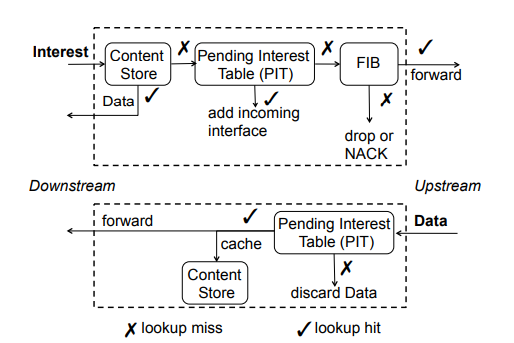
\includegraphics{Chapters/Figures/fowarding.png}
\caption{Processo de encaminhamento num nó \gls{NDN} \cite{papadopoulos_lixia_2014}}
\label{fig:Forwarding}
\end{figure}

Após a análise da imagem podemos retirar que o fluxo segue os seguintes passos:
\begin{enumerate}
    \item Receção do \textit{Interest}.
    \item Consulta da \textbf{Content Store}:
    \begin{itemize}
        \item se \textit{cache hit}: envia \textit{Data} pela interface de entrada.
        \item se \textit{cache miss}: avança para a PIT.
    \end{itemize}
    \item Consulta/atualização da \textbf{PIT}:
    \begin{itemize}
        \item se já existir uma entrada: adiciona-se a interface e descarta-se o Interest (evita duplicações).
        \item caso contrário: cria-se uma nova entrada.
    \end{itemize}
    \item Consulta da \textbf{FIB} para determinar o(s) próximo(s) salto(s).
    \item Reencaminhamento do \textit{Interest}.
    \item À chegada do pacote \textit{Data}:
    \begin{itemize}
        \item consulta-se a PIT para determinar as interfaces de saída;
        \item envia-se o \textit{Data} por todas as interfaces registadas;
        \item armazena-se o conteúdo na CS (política dependente do router);
        \item remove-se a entrada da PIT.
    \end{itemize}
\end{enumerate}


%%%%%%%%%%%%%%%%%%%%%%%%%%%%%%%%%%%%%%%%%%%%%%%%%%
\subsection{Mecanismos de caching e segurança}
\label{sub:NDN_cache_seguranca}
%%%%%%%%%%%%%%%%%%%%%%%%%%%%%%%%%%%%%%%%%%%%%%%%%%

\subsubsection{Caching distribuído}

O \gls{NDN} implementa \textit{in-network caching}, permitindo que qualquer router responda a um \textit{Interest} se tiver uma cópia válida do conteúdo. Este comportamento melhora substancialmente:
\begin{itemize}
    \item eficiência da rede;
    \item tolerância a falhas;
    \item desempenho em mobilidade.
\end{itemize}



\subsubsection{Segurança no NDN}

A segurança no NDN é \textbf{orientada aos dados}, e não aos canais.  
Cada pacote \textit{Data} inclui obrigatoriamente:

\begin{itemize}
    \item assinatura criptográfica do produtor;
    \item nome do dado;
    \item conteúdo e metadados.
\end{itemize}

Este mecanismo permite que os consumidores validem a autenticidade do conteúdo independentemente da fonte que o entregou (router, cache, produtor). A validação do nome e da assinatura é guiada por \textbf{trust schemas}, que definem regras estruturadas para relacionar nomes de conteúdos, identidades e chaves de assinatura.


%%%%%%%%%%%%%%%%%%%%%%%%%%%%%%%%%%%%%%%%%%%%%%%%%%
\subsection{Limitações do NDN em contextos móveis}
\label{sub:NDN_limitacoes_mobilidade}
%%%%%%%%%%%%%%%%%%%%%%%%%%%%%%%%%%%%%%%%%%%%%%%%%%

Apesar das vantagens, o NDN enfrenta limitações importantes em cenários altamente dinâmicos, como redes veiculares:

\begin{itemize}
    \item \textbf{Rutura do caminho inverso}: a entrega do \textit{Data} depende da validade da entrada na PIT, que assume que o percurso inverso continua disponível. Em mobilidade elevada, produtor e consumidor podem mover-se antes da chegada da resposta.
    \item \textbf{PIT flooding}: mobilidade provoca elevada taxa de timeouts e criação de novas entradas, aumentando risco de congestionamento.
    \item \textbf{Encaminhamento instável}: a FIB pode não refletir rapidamente as mudanças topológicas.
    \item \textbf{Desperdício de cache}: conteúdos relevantes podem ficar armazenados em nós que rapidamente se afastam da área onde são úteis.
\end{itemize}

Em redes veiculares, onde a conectividade é frequentemente intermitente e os nós são altamente móveis, estas propriedades tornam o \gls{NDN} uma base ideal para a disseminação cooperativa de informações. Quando um veículo solicita um conteúdo (por exemplo, um alerta de acidente ou dados de tráfego), qualquer outro nó que tenha armazenado previamente essa informação na sua \gls{CS} pode responder, sem necessidade de comunicação direta com o produtor original. Este comportamento distribuído e orientado ao conteúdo melhora a eficiência, reduz o tráfego redundante e aumenta a tolerância a falhas \cite{rahman_data-centric_2021, papadopoulos_-vehicle_2021}.

Além disso, o modelo de encaminhamento baseado em nomes facilita a agregação e filtragem de informações contextuais (por exemplo, \texttt{/ndn/highway/alert/km42}), permitindo disseminação seletiva e localizada, um requisito essencial para aplicações de segurança e gestão de tráfego em ambientes \gls{V2X}. Assim, o \GLS{NDN} fornece a base conceptual e técnica para a evolução das redes veiculares rumo ao paradigma \textbf{\gls{V-NDN}}, explorado na secção seguinte.

%%%%%%%%%%%%%%%%%%%%%%%%%%%%%%%%%%%%%%%%%%%%%%%%%%
\section{\emph{\gls{V-NDN}}}
\label{sub:VNDN}
%%%%%%%%%%%%%%%%%%%%%%%%%%%%%%%%%%%%%%%%%%%%%%%%%%

No contexto dos veículos conectados e das \gls{VANETs}, a mobilidade elevada, a topologia dinâmica e a conectividade intermitente tornam desafiadora a manutenção de ligações fim a fim robustas baseadas em endereços IP \cite{rahman_data-centric_2021}. Para responder a estas limitações, surge o paradigma \textbf{\gls{V-NDN}}, uma extensão natural da arquitetura \gls{NDN} orientada ao conteúdo, na qual a comunicação é guiada por nomes de dados e não por endereços de origem ou destino.

A comunicação deixa de depender de endereços e rotas estáticas, passando a ser guiada por \textbf{nomes de dados}, explorando \textit{Interest/Data packets}, \textit{in-network caching} e \textit{name-based forwarding}. No entanto, aplicar o \gls{NDN} ao domínio veicular implica resolver desafios específicos da mobilidade rápida, que afetam particularmente a \textbf{\gls{PIT}} e a \textbf{\gls{FIB}}, cujo estado pode tornar-se inválido antes da receção dos dados.

%%%%%%%%%%%%%%%%%%%%%%%%%%%%%%%%%%%%%%%%%%%%%%%%%%
\subsection{Motivação para V-NDN}
%%%%%%%%%%%%%%%%%%%%%%%%%%%%%%%%%%%%%%%%%%%%%%%%%%

Ao contrário do paradigma IP tradicional, o \gls{NDN} permite que os dados sejam requisitados pelo seu nome, independentemente da localização do produtor. Em contexto veicular, esta abordagem é especialmente vantajosa, pois:
\begin{itemize}
    \item evita dependência de ligações fim-a-fim frágeis;
    \item permite descoberta de conteúdo local através de \gls{V2V};
    \item explora mobilidade como mecanismo de transporte de dados (\textit{store-carry-forward});
    \item suporta comunicação resiliente em cenários com topologias altamente voláteis.
\end{itemize}

O paradigma \gls{V-NDN} aproveita ainda o \textit{in-network caching} para disponibilizar informação crítica, como alertas de colisão ou condições da via sem necessidade de recorrer a \gls{RSUs} ou a servidores centrais.

%%%%%%%%%%%%%%%%%%%%%%%%%%%%%%%%%%%%%%%%%%%%%%%%%%
\subsection{Mecanismos adaptados de encaminhamento}
%%%%%%%%%%%%%%%%%%%%%%%%%%%%%%%%%%%%%%%%%%%%%%%%%%

O encaminhamento baseado em nomes do \gls{NDN} necessita de adaptações significativas para funcionar em mobilidade extrema. Em redes veiculares, os problemas mais evidentes incluem:
\begin{itemize}
    \item \textbf{invalidação rápida de entradas na \gls{PIT}} devido ao movimento dos nós antes da receção do pacote \textit{Data};
    \item \textbf{obsolescência da \gls{FIB}}, cujo conjunto de nexthops deixa de refletir a topologia atual;
    \item \textbf{broadcast excessivo}, gerando conteúdo redundante e colisões.
\end{itemize}

Para mitigar estas limitações, a literatura propõe várias estratégias específicas de \gls{V-NDN}:

\subsubsection*{Forwarding oportunístico}
Os interesses são reenviados por qualquer nó que apresente melhores condições momentâneas de conectividade. O processo explora oportunidades de contacto, reduzindo a dependência de rotas estáveis
\subsubsection*{Forwarding geográfico}
A decisão de encaminhamento usa a posição, velocidade e direção do veículo. Esta técnica permite reduzir o espaço de procura e limita a difusão de interesses a regiões relevantes \cite{aldahlan_geographic_2019}.

\subsubsection*{Seleção de nós dominantes}
Alguns nós são escolhidos como retransmissores preferenciais (por exemplo, veículos mais centrais na topologia ou com maior grau de conetividade). A técnica reduz duplicação de mensagens e colisões, melhorando a eficiência

%%%%%%%%%%%%%%%%%%%%%%%%%%%%%%%%%%%%%%%%%%%%%%%%%%
\subsection{Caching distribuído e cooperativo}
%%%%%%%%%%%%%%%%%%%%%%%%%%%%%%%%%%%%%%%%%%%%%%%%%%

A \gls{CS} desempenha um papel fundamental no \gls{V-NDN}, pois permite:
\begin{itemize}
    \item reduzir latência através de respostas locais;
    \item aumentar a disponibilidade de dados em regiões com baixa densidade;
    \item evitar retransmissões desnecessárias ao produtor original.
\end{itemize}

Estratégias de \textbf{caching cooperativo} (por exemplo, \cite{amadeo_caching_2020}) incluem:
\begin{itemize}
    \item partilha de metadados sobre conteúdos armazenados;
    \item coordenação entre veículos para evitar armazenamento redundante;
    \item políticas adaptadas de substituição (LRU/LFU/contexto veicular);
    \item associação do cache ao movimento do veículo (conteúdo “transportado” fisicamente).
\end{itemize}

Assim, os veículos tornam-se distribuidores móveis de informação, ampliando a eficácia do paradigma.

%%%%%%%%%%%%%%%%%%%%%%%%%%%%%%%%%%%%%%%%%%%%%%%%%%
\subsection{Limitações atuais da V-NDN}
%%%%%%%%%%%%%%%%%%%%%%%%%%%%%%%%%%%%%%%%%%%%%%%%%%

Apesar das vantagens, subsistem desafios importantes:
\begin{itemize}
    \item \textbf{volatilidade extrema}, que provoca expiração prematura de entradas na \gls{PIT};
    \item \textbf{dinâmica da \gls{FIB}}, que necessita de atualizações frequentes e não escaláveis em grandes cenários;
    \item \textbf{gestão de congestionamento e duplicação}, particularmente crítica em broadcast;
    \item vulnerabilidade a ataques como \textit{Interest Flooding};
    \item impacto de cenários urbanos complexos, com sombra e irregularidade de densidade veicular.
\end{itemize}

Estas limitações demonstram que o \gls{V-NDN} requer ainda investigação em mecanismos de segurança, coordenação de caches e encaminhamento inteligente.

%%%%%%%%%%%%%%%%%%%%%%%%%%%%%%%%%%%%%%%%%%%%%%%%%%
\subsection{Trabalhos relevantes sobre disseminação de informação em V-NDN}
%%%%%%%%%%%%%%%%%%%%%%%%%%%%%%%%%%%%%%%%%%%%%%%%%%
Diversos estudos têm explorado o paradigma \gls{V-NDN} com o objetivo de melhorar a disseminação de conteúdos em ambientes veiculares altamente dinâmicos. As abordagens existentes podem ser agrupadas em três grandes categorias: estratégias de encaminhamento adaptativo, mecanismos de cache colaborativo e soluções voltadas à segurança e gestão de mobilidade.

\subsubsection{Encaminhamento e mobilidade}
O encaminhamento em \gls{V-NDN} é um dos aspetos mais investigados, dada a necessidade de garantir entrega eficiente de dados em topologias em constante mudança. Em \cite{cha_mobility_2017}, os autores propõem um serviço de mobilidade para consumidores em \gls{NDN}, permitindo que um consumidor reemita um interesse mesmo após mudanças de localização, facilitando a continuidade da comunicação em ambientes móveis.  
Além disso, mecanismos de priorização de interesses e redução de duplicação de pedidos têm sido estudados, de modo a otimizar a utilização da largura de banda e reduzir atrasos em cenários com alta densidade veicular.

\subsubsection{Cache colaborativo e eficiência de disseminação}  
A otimização do uso da \gls{CS} em cada nó é outra linha de investigação relevante. Em \cite{amadeo_caching_2020}, é proposto um esquema de cache cooperativo, onde os veículos partilham informações sobre os conteúdos armazenados, permitindo respostas rápidas a interesses repetidos.
Para compreender o funcionamento do esquema, é importante detalhar:
\begin{itemize}
\item Algoritmos de gestão do cache (por exemplo, LRU, LFU ou variantes específicas para \gls{V-NDN});
\item Tipo de metadados partilhados e periodicidade das mensagens de sincronização;
\item Critérios utilizados para decidir qual veículo responde a um interesse.
\end{itemize}
A distribuição inteligente de conteúdos reduz o consumo de largura de banda e melhora a disponibilidade de dados em zonas de baixa densidade.
Um exemplo concreto deste tipo de abordagem é discutido em \cite{amadeo_caching_2020}, onde conteúdos transitórios, como alertas de travagem brusca ou variações rápidas de velocidade são armazenados cooperativamente pelos veículos que passam pela zona afetada. Assim, mesmo após o veículo que gerou o alerta já ter abandonado a área, os nós vizinhos conseguem responder rapidamente a novos interesses, garantindo que os veículos a montante recebem a informação crítica com baixa latência, mesmo em cenários de conectividade intermitente.

\subsubsection{Gestão de mobilidade e segurança}  
A mobilidade dos nós e a volatilidade das ligações representam desafios adicionais para manter a consistência e autenticidade dos dados. Em \cite{cha_mobility_2017}, os autores discutem a integração de mecanismos de autenticação leve nos pacotes de dados do \gls{V-NDN}, utilizando assinaturas baseadas em nomes hierárquicos.  
Aspectos a destacar incluem:
\begin{itemize}
    \item Processo de assinatura hierárquica e verificação nos nós veiculares;
    \item Gestão das chaves hierárquicas e distribuição segura;
    \item Comparação com autenticação tradicional do \gls{NDN}, em termos de overhead computacional.
\end{itemize}
Esta abordagem garante integridade e autenticidade sem introduzir sobrecarga significativa.
\subsection{Estruturas Hierárquicas e Clustering em \gls{V-NDN}}
\label{sec:hierarquia-vndn}

Modelos hierárquicos baseados em \textit{clustering}, como o \gls{PACM} \cite{sampath_position-based_2021}, 
organizam os veículos em grupos estruturados para facilitar a disseminação de dados. Ao utilizar a posição 
como critério de agrupamento, estes sistemas oferecem maior estabilidade na comunicação dentro de 
clusters e podem servir como base para mecanismos escaláveis em redes veiculares.

A literatura recente demonstra que estruturas hierárquicas são particularmente eficazes em ambientes 
de elevada mobilidade, pois permitem reduzir a complexidade da comunicação ao nível local antes da 
agregação global. Trabalhos como \cite{de_castro_dynamic_2015} propõem arquiteturas hierárquicas 
dinâmicas especificamente orientadas a NDN em cenários veiculares, evidenciando que a 
agregação local de informação e a existência de líderes de cluster podem reduzir a redundância de 
mensagens e melhorar a estabilidade da comunicação.

De forma complementar, surveys como \cite{ayyub_comprehensive_2022} destacam que clusters 
geograficamente estáveis aumentam a longevidade das ligações e reduzem a oscilação do estado, 
características essenciais para a resiliência e eficiência da disseminação de conteúdos em ambientes 
veiculares altamente dinâmicos.

\subsection{Síntese}
De modo geral, a literatura demonstra que o \gls{V-NDN} é capaz de melhorar a eficiência da disseminação de conteúdos, explorando os princípios de \textit{in-network caching} e \textit{name-based forwarding} do \gls{NDN}, ainda assim indica que o \gls{V-NDN} tem potencial para superar limitações das redes \gls{V2X} tradicionais, oferecendo um modelo mais resiliente e orientado ao conteúdo.
As estratégias adaptativas de encaminhamento e cache mostram-se promissoras para lidar com mobilidade elevada e topologias esparsas, mas persistem desafios relacionados com a gestão de segurança, sincronização de caches e balanceamento de tráfego.  
O desenvolvimento de mecanismos combinados, que integrem encaminhamento adaptativo, cache cooperativo e autenticação leve, constitui uma tendência atual de investigação em \gls{V-NDN}.

%%%%%%%%%%%%%%%%%%%%%%%%%%%%%%%%%%%%%%%%%%%%%%%%%%
\section{Sincronização de Bases de Dados}
\label{sec:sync_distrib}
%%%%%%%%%%%%%%%%%%%%%%%%%%%%%%%%%%%%%%%%%%%%%%%%%%

A sincronização de bases de dados distribuídas visa garantir que múltiplos nós, potencialmente dispersos geograficamente e sujeitos a falhas de comunicação, mantêm uma visão coerente de um conjunto de dados partilhado. Em ambientes estáveis, esta sincronização pode ser assegurada através de mecanismos centralizados ou com garantias fortes de consistência. No entanto, em redes móveis, intermitentes e sem infraestruturas como as \glspl{VANETs} este problema torna-se substancialmente mais complexo.

Nesta secção apresentam-se os princípios fundamentais da sincronização distribuída, modelos de consistência, e os protocolos clássicos que servem de base conceptual para os mecanismos de sincronização em \gls{NDN}. Estes conceitos são essenciais para compreender a evolução e o funcionamento de protocolos como o \gls{DSSN}, \gls{DDSN} e, finalmente, o \gls{SVSync}.

%%%%%%%%%%%%%%%%%%%%%%%%%%%%%%%%%%%%%%%%%%%%%%%%%%
\subsection{Conceitos Gerais de Sincronização Distribuída}
\label{sub:conc_gerais_sync}
%%%%%%%%%%%%%%%%%%%%%%%%%%%%%%%%%%%%%%%%%%%%%%%%%%

A sincronização distribuída procura assegurar que múltiplos repositórios de dados evoluem de forma coerente ao longo do tempo, mesmo quando cada nó observa apenas uma parte do estado global. Os desafios clássicos incluem:

\begin{itemize}
    \item \textbf{Latências variáveis:} diferentes caminhos na rede conduzem a tempos de propagação distintos;
    \item \textbf{Partições de rede e churn:} nós podem entrar e sair constantemente;
    \item \textbf{Atualizações concorrentes:} múltiplos produtores podem gerar versões distintas de um mesmo objeto;
    \item \textbf{Links instáveis:} presentes especialmente em redes ad-hoc e veiculares.
\end{itemize}

Para resolver estes desafios, diversas estruturas de metadados foram propostas, como vetores de versão, relógios lógicos ou timestamps híbridos. Estes mecanismos permitem identificar causalidade entre eventos e detetar divergências entre réplicas.

%%%%%%%%%%%%%%%%%%%%%%%%%%%%%%%%%%%%%%%%%%%%%%%%%%
\subsection{Modelos de Consistência}
\label{sub:modelos_consistencia}
%%%%%%%%%%%%%%%%%%%%%%%%%%%%%%%%%%%%%%%%%%%%%%%%%%

Os modelos de consistência definem as garantias observáveis pelos clientes no que respeita à ordem e visibilidade das atualizações.

\subsubsection*{Consistência Forte}
Garante que todas as réplicas observam exatamente o mesmo estado a qualquer instante, frequentemente através de mecanismos de bloqueio, consenso (e.g., Paxos, Raft) ou coordenação centralizada. Embora desejável, é impraticável em redes móveis devido ao elevado custo de coordenação e à sensibilidade a partições.

\subsubsection*{Consistência Eventual}
Assegura que, na ausência de novas atualizações e assumindo alguma conectividade, todas as réplicas convergem para o mesmo estado. Este modelo é mais adequado a redes veiculares, onde falhas de ligação são frequentes.

\subsubsection*{Consistência Causal}
Garante que relações de dependência entre atualizações são preservadas. Vetores de versão e relógios lógicos são mecanismos típicos para atingir esta consistência, equilibrando custo e precisão.

%%%%%%%%%%%%%%%%%%%%%%%%%%%%%%%%%%%%%%%%%%%%%%%%%%
\subsection{Protocolos Clássicos de Sincronização}
\label{sub:protocolos_classicos}
%%%%%%%%%%%%%%%%%%%%%%%%%%%%%%%%%%%%%%%%%%%%%%%%%%

Antes da evolução para mecanismos específicos de \gls{NDN}, vários protocolos foram desenvolvidos com o objetivo de sincronizar conjuntos de dados de forma eficiente.

\subsubsection*{Vetores de Versão}
Os vetores de versão permitem representar o estado de cada produtor através de números de sequência. A comparação entre vetores possibilita a deteção imediata de dados em falta. São a base conceptual dos vetores de estado utilizados em \gls{DSSN}, \gls{DDSN} e \gls{SVSync}.

\subsubsection*{Pub/Sub}
Modelos de \textit{publish/subscribe} fornecem uma forma eficaz de disseminar atualizações, mas dependem tipicamente de brokers ou overlays estáveis, o que os torna pouco adequados a redes altamente móveis.

\subsubsection*{Flooding Confiável}
Técnicas de flooding com mecanismos de supressão ou retransmissão controlada garantem disseminação rápida, mas geram overhead elevado em redes densas.

%%%%%%%%%%%%%%%%%%%%%%%%%%%%%%%%%%%%%%%%%%%%%%%%%%
\subsection{Requisitos de Sincronização em Ambientes Veiculares}
\label{sub:requisitos_veiculares}
%%%%%%%%%%%%%%%%%%%%%%%%%%%%%%%%%%%%%%%%%%%%%%%%%%

As redes veiculares (\gls{V2V}, \gls{V2X}) apresentam características extremas:

\begin{itemize}
    \item \textbf{Mobilidade elevada:} ligações com durações de poucos segundos;
    \item \textbf{Churn intenso:} conjunto de vizinhos muda constantemente;
    \item \textbf{Latência crítica:} informação como alertas de segurança deve ser disseminada rapidamente;
    \item \textbf{Baixo overhead:} excesso de tráfego compromete segurança e QoS.
\end{itemize}

Estes requisitos motivaram o desenvolvimento de mecanismos de sincronização adaptados ao paradigma \gls{NDN}, culminando na evolução 
\gls{DSSN} → \gls{DDSN} → \gls{SVSync}.

%%%%%%%%%%%%%%%%%%%%%%%%%%%%%%%%%%%%%%%%%%%%%%%%%%
\section{\emph{Sincronização no \gls{NDN}}}
\label{sub:Sinc__NDN}
%%%%%%%%%%%%%%%%%%%%%%%%%%%%%%%%%%%%%%%%%%%%%%%%%%

O objetivo da sincronização no NDN é garantir que todos os participantes mantêm uma visão atualizada e consistente do conjunto de dados partilhado. Para isso, cada nó precisa de identificar quais são os dados que lhe faltam, ou seja, quais são os dados que foram recentemente produzidos e atualizados por outros membros do grupo. Cada utilizador transmite o seu Estado para os outros participantes através de trocas de Interesse-Dados. Esta troca pode ser feita de duas formas: o produtor envia ativamente notificações sobre o seu estado, ou cada utilizador consulta periodicamente o grupo de sincronização.

Uma abordagem possível para a sincronização em \gls{NDN} é o uso de vetores de estado. A ideia central é representar o estado de um conjunto de dados na forma de um vetor de versões, onde cada componente indica o prefixo de um produtor e o número de sequência dos seus dados mais recentes (conforme ilustrado na Figura \ref{fig:SV}). Como um vetor de estado enumera explicitamente a versão mais recente de cada produtor, as diferenças nos conjuntos de dados podem ser identificadas fazendo uma simples comparação entre os valores de cada prefixo. Para atualizar o seu Vetor de Estado, o nó adota o maior número de sequência disponível para cada produtor. O facto de a representação do estado baseada em Vetores de Estado permitir uma comparação direta do estado, permite que os nós identifiquem diretamente os dados em falta sem necessidade de trocas de mensagens adicionais. Esta característica torna esta abordagem especialmente adequada para redes ad-hoc, onde grandes divergências de estado são bastante comuns. O tamanho do Vetor cresce proporcionalmente ao número de produtores cujos estados precisam ser trocados. Contudo, a listagem explícita dos estados de cada produtor permite a transmissão de Vetores de Estado parciais quando há restrições no tamanho dos pacotes.

\begin{figure}[H]
    \centering
    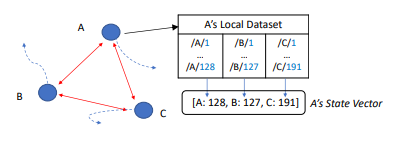
\includegraphics{Chapters/Figures/svs.png}
    \caption{Exemplo de Vetor de Estado \cite{li_brief_2018}} 
    \label{fig:SV}   
\end{figure}

Como o \gls{NDN} foi concebido para suportar comunicações assíncronas, exigir uma consistência perfeita das informações de associação entre todos os membros do grupo não é viável. Para contornar esta limitação, a sincronização por Vetores de Estado foi rapidamente sucedida por outro protocolo de sincronização: o \gls{DSSN}. O \gls{DSSN} introduz uma alteração simples, mas crucial, nos vetores de estado clássicos, permitindo a sincronização eficiente de conjuntos de dados em grupos de sensores que entram periodicamente em estados de inatividade. A principal novidade do \gls{DSSN} consiste na reformulação do vetor de estado: em vez de ser apenas uma lista de números de sequência, cada elemento passa a ser uma tupla [prefixo do participante, número de sequência], transportada diretamente em cada Interesse de Sincronização. Este formato codifica de forma explícita o estado global do conjunto de dados partilhado, permitindo que qualquer nó destinatário interprete corretamente o estado, mesmo em situações de inconsistência elevada entre os participantes \cite{li_data_2018}.

Em comparação com o vetor de estado tradicional apresentado na Figura \ref{fig:SV}, a inovação do \gls{DSSN} está na capacidade de lidar com participantes intermitentes e de transmitir informação de estado global de forma compacta e consistente, sem necessidade de mensagens adicionais para reconciliação de dados. Por outro lado, o \gls{DDSN} é uma extensão do \gls{DSSN} focada em ambientes com mobilidade e topologias mais dinâmicas, introduzindo mecanismos adaptativos para manter a consistência do estado mesmo quando a conectividade entre nós é altamente variável. O \gls{DDSN} introduziu uma série de melhorias, incluindo:

\begin{itemize}
    \item 1. Priorização de transmissão que permite determinar quais mensagens devem ser enviadas primeiro durante períodos de conectividade transitória.
    \item 2. Modo inativo que reduz o tráfego de sincronização e otimiza o consumo de energia quando não há outros nós dentro da área de comunicação.
\end{itemize}

Apesar da sua eficiência em ambientes altamente dinâmicos e disruptivos, o \gls{DDSN} tem um desempenho inferior em redes bem conectadas, devido à sua ênfase exclusiva em cenários com conectividade instável. A experiência adquirida com os protocolos anteriores levou ao desenvolvimento do \gls{SVSync}. Este protocolo herda a codificação do vetor de estado introduzida pelo \gls{DSSN}, mas elimina funcionalidades específicas para redes de sensores e ambientes com elevada disrupção. **Importa salientar que o SVSync não foi concebido para cenários veiculares ou para \gls{V-NDN}, sendo um protocolo de sincronização genérico para grupos NDN.**

\vspace{0.3cm}

%%%%%%%%%%%%%%%%%%%%%%%%%%%%%%%%%%%%%%%%%%%%%%%%%%
\subsection{\emph{\gls{SVSync}}}
\label{sub:Sinc_NDN_refined}
%%%%%%%%%%%%%%%%%%%%%%%%%%%%%%%%%%%%%%%%%%%%%%%%%%

O \gls{SVSync} adota uma estratégia de codificação de estado distinta. O seu design segue a convenção de nomeação sequencial dos dados e transporta diretamente a representação do namespace do conjunto de dados, codificada em pares [nome do produtor, número de sequência] (Figura \ref{fig:SVs}), dentro de cada Interesse Sync Multicast. A decisão de design do \gls{SVSync} de incluir o namespace do conjunto de dados bruto em cada Interesse de Sincronização oferece uma vantagem significativa: qualquer nó que receba o Interesse compreende de imediato o estado do conjunto de dados, independentemente do seu próprio estado atual ou de eventuais mensagens perdidas anteriormente. No entanto, permitir que um Interesse recebido possa alterar o estado de um participante abre a porta a possíveis abusos. Para mitigar esse risco, o \gls{SVSync} exige que todos os Interesses de Sincronização sejam assinados.

\begin{figure}[h]
\centering
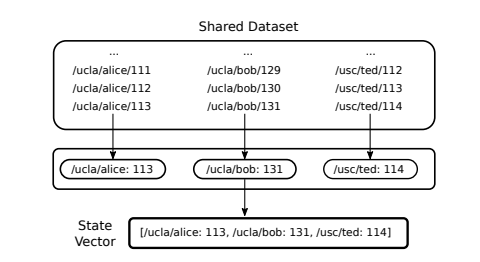
\includegraphics{Chapters/Figures/vsvsync.png}
\caption{Exemplo de Vetor de Estado \cite{moll_brief_nodate}}
\label{fig:SVs}
\end{figure}

\subsubsection{Funcionamento do \gls{SVSync}}
Cada grupo de sincronização utiliza um prefixo multicast de grupo, garantindo que todos os participantes recebam as mensagens de sincronização. Cada nó possui também um prefixo de publicação próprio, sob o qual os seus dados ficam acessíveis aos restantes participantes.

O \gls{SVSync} utiliza apenas um tipo de mensagem: o \textit{Interest}. Estes interesses são enviados em duas situações principais:

\begin{itemize}
\item \textbf{Eventos:} sempre que há uma alteração no estado do conjunto de dados, os participantes notificam imediatamente os restantes.
\item \textbf{Envios periódicos:} garantem consistência do conjunto de dados, mesmo em caso de perda de pacotes ou desconexões temporárias.
\end{itemize}

Os interesses ativados por eventos permitem a rápida disseminação de informações, enquanto os envios periódicos mantêm todos os participantes sincronizados, mitigando divergências temporárias. O fluxograma apresentado na Figura~\ref{fig:SVsyync} ilustra o funcionamento do protocolo \gls{SVSync} na partilha e sincronização do estado entre os participantes. Cada nó, ao detetar uma alteração no seu estado local, gera um interesse de sincronização contendo o novo vetor de estado (par nome-produtor, número de sequência), que é enviado por multicast a todos os membros do grupo. Paralelamente, mesmo na ausência de eventos, cada nó envia de forma periódica estes interesses para garantir a convergência do estado global, mitigando os efeitos de perdas de pacotes ou desconexões temporárias.

Ao receber um interesse de sincronização, cada participante compara o vetor de estado recebido com o seu próprio estado atual. Caso identifique diferenças, solicita diretamente os dados em falta usando o mecanismo de interesse do \gls{NDN}, garantindo assim a atualização eficiente e atempada de todos os membros do grupo. O processo repete-se ciclicamente, assegurando que novas atualizações são prontamente disseminadas e integradas por todos os participantes.

Em síntese, o fluxograma evidencia as duas fontes principais de emissão dos interesses (evento e período), a receção e análise desses interesses, e as ações subsequentes de pedido dos dados em falta. Este ciclo contínuo é a base da robustez do \gls{SVSync}, permitindo elevada consistência dos dados partilhados mesmo em redes dinâmicas e sujeitas a desconexões frequentes, como é o caso das redes veiculares.

\begin{figure}[H]
\centering
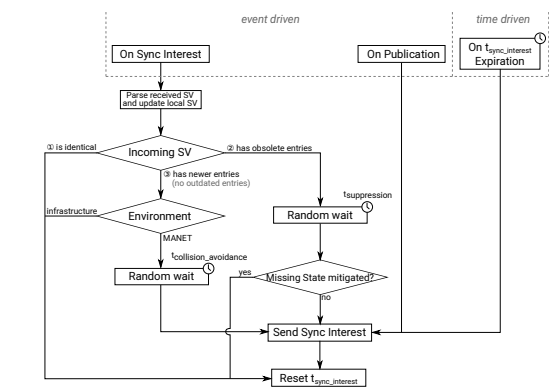
\includegraphics{Chapters/Figures/Captura de ecrã 2025-03-24 160649.png}
\caption{Fluxograma do funcionamento do \gls{SVSync} \cite{moll_brief_nodate}}
\label{fig:SVsyync}
\end{figure}

O SVSync utiliza os interesses apenas como notificações unidirecionais, sem gerar respostas imediatas. Isso evita problemas de múltiplos produtores respondendo ao mesmo interesse, mas apresenta algumas limitações importantes, especialmente em cenários de mobilidade elevada:

\paragraph{Limitações do SVSync}
\begin{itemize}
\item \textbf{\gls{PIT} persistente elevado:} cada interesse \textit{multicast} permanece pendente em todos os encaminhadores até expirar, aumentando o uso de memória em redes densas.
\item \textbf{Entrega parcial de atualizações:} devido ao princípio \textit{um interesse, um dado}, diferentes participantes podem receber subconjuntos distintos de atualizações, resultando em divergência temporária de estado.
\item \textbf{Dependência de conectividade regular:} em cenários com nós móveis ou desconexões frequentes (como em \gls{V-NDN}), a falta de retransmissão automática pode atrasar a convergência global.
\item \textbf{Escalabilidade limitada:} o crescimento do grupo aumenta linearmente o número de interesses necessários para manter o estado atualizado, afetando a eficiência em redes grandes.
\end{itemize}

\vspace{0.15cm}


\paragraph{ChronoSync e PSync no contexto da sincronização NDN}

Embora o foco principal desta secção seja o SVSync e os protocolos que lhe deram origem, existem outros protocolos amplamente utilizados no NDN que merecem referência, pois têm sido considerados para sincronização em cenários móveis.

O \textbf{ChronoSync} utiliza um \emph{digest tree} para representar o estado global e detetar diferenças entre produtores, recorrendo a sincronização incremental sempre que o digest muda. Esta abordagem é eficiente quando a conectividade é relativamente estável, mas sofre quebras significativas quando a vizinhança muda rapidamente, como acontece em redes veiculares \cite{zhu_lets_2013}.

Já o \textbf{PSync} combina vetores de estado com estruturas compactas como os \emph{Invertible Bloom Lookup Tables (IBLTs)}, permitindo sincronização parcial e escalável entre grandes grupos de produtores. No entanto, como o desempenho dos IBLTs depende de estimativas corretas do tamanho do conjunto, variações abruptas de vizinhança, típicas de \gls{V-NDN}, levam a erros de decodificação e necessidade de retransmissões adicionais \cite{dragoi_psync_2016}.

Estes dois protocolos, embora eficientes em redes moderadamente dinâmicas, não conseguem garantir convergência rápida e estável em cenários de mobilidade extrema.

%%%%%%%%%%%%%%%%%%%%%%%%%%%%%%%%%%%%%%%%%%%%%%%%%%
\subsection{Comparação de Protocolos de Sincronização}
\label{sub:sync_comparison}
%%%%%%%%%%%%%%%%%%%%%%%%%%%%%%%%%%%%%%%%%%%%%%%%%%

Para compreender melhor as diferenças entre abordagens de sincronização, apresentamos uma análise comparativa entre os protocolos \gls{DSSN}, \gls{DDSN} e \gls{SVSync}, seguida de uma visão sobre protocolos hierárquicos aplicados a redes IoT e \gls{VANETs}.

\subsubsection{DSSN}
\label{subsub:dssn}

O protocolo \gls{DSSN} \Cite{xu_achieving_2018} utiliza vetores de estado codificados em tuplas do tipo 
\texttt{[prefixo, número-de-sequência]}, permitindo que cada nó compare
diretamente o seu estado local com o estado recebido. Esta abordagem é robusta
a conectividade intermitente e adequada a redes de sensores, embora apresente
limitações de escalabilidade.

\begin{algorithm}[H]
\caption{Processo de sincronização no DSSN}
\begin{algorithmic}[1]
\Procedure{SendSyncInterest}{}
    \State interest.payload $\gets$ LocalStateVector
    \State \textbf{broadcast}(interest)
\EndProcedure

\Statex

\Procedure{OnReceiveSyncInterest}{RemoteVector}
    \State MissingData $\gets \emptyset$
    \ForAll{(prefix, remoteSeq) $\in$ RemoteVector}
        \State localSeq $\gets$ LocalStateVector[prefix]
        \If{remoteSeq $>$ localSeq}
            \State MissingData $\gets$ MissingData $\cup$ (prefix, localSeq+1..remoteSeq)
        \EndIf
    \EndFor
    \If{MissingData $\neq \emptyset$}
        \State \Call{RequestMissingData}{MissingData}
    \EndIf
\EndProcedure

\Statex

\Procedure{RequestMissingData}{MissingData}
    \ForAll{(prefix, seqRange) $\in$ MissingData}
        \ForAll{seq $\in$ seqRange}
            \State sendInterest(prefix/seq)
        \EndFor
    \EndFor
\EndProcedure

\Statex

\Procedure{OnReceiveData}{prefix, seq}
    \State store(data)
    \If{seq $>$ LocalStateVector[prefix]}
        \State LocalStateVector[prefix] $\gets$ seq
    \EndIf
\EndProcedure
\end{algorithmic}
\end{algorithm}

\subsubsection{DDSN}
\label{subsub:ddsn}

O protocolo \gls{DDSN} \cite{li_distributed_2019} estende o \gls{DSSN} e introduz dois mecanismos
adicionais: (i) \textit{prioritização} de dados em falta, e (ii) modo
\textit{inativo} que reduz a sobrecarga quando o nó não tem vizinhos. O vetor de
estado mantém o mesmo formato do DSSN, mas o processo de disseminação adapta-se
à mobilidade e instabilidade da conectividade.

\begin{algorithm}[H]
\caption{Processo de sincronização no DDSN}
\begin{algorithmic}[1]
\State Mode $\in$ \{ACTIVE, SLEEP\}

\Statex

\Procedure{PeriodicCheckNeighbors}{}
    \If{NeighborSet é vazio}
        \State Mode $\gets$ SLEEP
    \Else
        \State Mode $\gets$ ACTIVE
    \EndIf
\EndProcedure

\Statex

\Procedure{SendSyncInterest}{}
    \State interest.payload $\gets$ LocalStateVector
    \If{Mode = ACTIVE}
        \State \textbf{broadcast}(interest)
    \Else
        \State \textbf{probabilisticBroadcast}(interest, $p_{low}$)
    \EndIf
\EndProcedure

\Statex

\Procedure{OnReceiveSyncInterest}{RemoteVector, Sender}
    \State NeighborSet.add(Sender)
    \State MissingData $\gets \emptyset$
    \ForAll{(prefix, remoteSeq) $\in$ RemoteVector}
        \State localSeq $\gets$ LocalStateVector[prefix]
        \If{remoteSeq $>$ localSeq}
            \State urgency $\gets$ remoteSeq - localSeq
            \State MissingData.add((prefix, localSeq+1..remoteSeq, urgency))
        \EndIf
    \EndFor
    \If{MissingData $\neq \emptyset$}
        \State \Call{PrioritizedRequest}{MissingData}
    \EndIf
\EndProcedure

\Statex

\Procedure{PrioritizedRequest}{MissingData}
    \State sort MissingData by urgency descending
    \ForAll{(prefix, seqRange, urgency) $\in$ MissingData}
        \ForAll{seq $\in$ seqRange}
            \State sendInterest(prefix/seq)
        \EndFor
    \EndFor
\EndProcedure

\end{algorithmic}
\end{algorithm}


\subsubsection{\gls{DSSN} vs \gls{DDSN} vs \gls{SVSync}}
\label{subsub:dssn_ddsn_svsync}
%%%%%%%%%%%%%%%%%%%%%%%%%%%%%%%%%%%%%%%%%%%%%%%%%%

Os protocolos \gls{DSSN}, \gls{DDSN} e \gls{SVSync} compartilham a ideia de vetores de estado para sincronização, mas diferem no foco e na adaptação a redes dinâmicas:

\begin{itemize}
    \item \textbf{\gls{DSSN}:} ideal para redes de sensores com conectividade intermitente. Permite a sincronização de conjuntos de dados em estados de inatividade, utilizando vetores de estado codificados em tuplas [prefixo, número de sequência]. Limitado em escalabilidade e em redes densas.
    
    \item \textbf{\gls{DDSN}} extensão do DSSN para redes ad-hoc sem fio, priorizando transmissão em períodos de conectividade transitória e modo inativo para reduzir tráfego. Desempenho inferior em redes bem conectadas \cite{rahman_analysis_2021}.
    
    \item \textbf{\gls{SVSync}:} mantém a codificação de vetores de estado do \gls{DSSN}, mas elimina funcionalidades específicas para sensores e adapta-se a redes mais dinâmicas. Limitações incluem overhead de \gls{PIT} persistente, divergência temporária de estado e escalabilidade limitada \cite{moll_brief_nodate}.
\end{itemize}

%%%%%%%%%%%%%%%%%%%%%%%%%%%%%%%%%%%%%%%%%%%%%%%%%%
\subsubsection{Protocolos hierárquicos em IoT e VANETs}
\label{subsub:hierarchical_sync}
%%%%%%%%%%%%%%%%%%%%%%%%%%%%%%%%%%%%%%%%%%%%%%%%%%

Outra abordagem relevante é a sincronização hierárquica, utilizada em redes IoT e \gls{VANETs}, onde um nó pivô coordena a disseminação de atualizações a subgrupos de nós. Esta estratégia reduz \textit{overhead} de comunicação e melhora a escalabilidade em topologias dinâmicas.

\begin{table}[h]
\centering
\caption{Protocolos hierárquicos de sincronização}
\label{tab:hier_sync}
\resizebox{\textwidth}{!}{%
\begin{tabular}{|l|c|c|c|c|}
\hline
Protocolo & Topologia & Métrica principal & Overhead & Aplicação \\ \hline
HierSync IoT \cite{luo_hierarchical_2025} & Redes de sensores & Latência & Baixo & IoT com grande número de nós \\ \hline
HierSync VANET & Redes veiculares & Entrega de dados & Médio & Disseminação de alertas e dados em V2V \\ \hline
\end{tabular}%
}
\end{table}

Estes protocolos hierárquicos são particularmente úteis em cenários onde a sincronização total direta seria inviável, como grupos grandes de sensores ou frotas de veículos conectados. Permitem que o pivô distribua o estado global enquanto os subgrupos replicam localmente, reduzindo latência e divergência entre nós.

%%%%%%%%%%%%%%%%%%%%%%%%%%%%%%%%%%%%%%%%%%%%%%%%%%
\subsection{Síntese crítica e lacunas}
\label{sec:critica}
%%%%%%%%%%%%%%%%%%%%%%%%%%%%%%%%%%%%%%%%%%%%%%%%%%

A análise dos protocolos de sincronização (\gls{DSSN}, \gls{DDSN}, \gls{SVSync}, ChronoSync e PSync) e das abordagens hierárquicas em IoT e \gls{VANETs} evidencia várias lacunas:

\begin{itemize}
    \item \textbf{Divergência de estado em redes móveis:} Protocolos como \gls{SVSync} mantêm \gls{PIT} persistente e podem gerar divergências temporárias de estado, especialmente em cenários com alta mobilidade veicular.
    \item \textbf{Escalabilidade limitada:} Muitos métodos funcionam bem em pequenos grupos, mas apresentam overhead elevado em redes grandes e altamente dinâmicas.
    \item \textbf{Falta de otimização para cenários veiculares:} Protocolos como ChronoSync e PSync assumem estabilidade temporal na vizinhança, o que não se verifica em \gls{V-NDN}.
    \item \textbf{Sincronização com conectividade intermitente:} O SVSync e protocolos similares não integram plenamente estratégias de retransmissão oportunista ou caching distribuído para aumentar a taxa de entrega em redes com desconexões frequentes.
    \item \textbf{Segurança e integridade:} Embora o SVSync utilize assinaturas, a mitigação de ataques como \emph{Interest Flooding} não é totalmente explorada nas abordagens de sincronização.
\end{itemize}

Estas lacunas motivam a proposta deste trabalho, que pretende:

\begin{itemize}
    \item Adaptar \gls{SVSync} para redes veiculares, combinando cache distribuído, retransmissão oportunista e priorização de interesses.
    \item Reduzir divergência de estado e overhead do \gls{PIT} em topologias dinâmicas.
    \item Avaliar o desempenho em cenários realistas de \gls{VANETs}, simulando alta mobilidade e densidade variável de veículos.
\end{itemize}

\section{Sincronização de Informação em \gls{V-NDN}}
\label{sec:sync-vndn}

A sincronização de informação em \gls{V-NDN}, como já vimos, constitui um desafio técnico
particularmente exigente, devido à elevada mobilidade dos veículos, à conectividade intermitente e à
variação constante da topologia. Neste contexto, mecanismos tradicionais de sincronização concebidos
para redes fixas, ou com mobilidade reduzida, revelam-se insuficientes. Esta secção apresenta uma
revisão aprofundada dos principais trabalhos dedicados à sincronização de dados em ambientes V-NDN.

Apesar da crescente adoção do paradigma \gls{NDN} em cenários veiculares, os mecanismos de 
sincronização continuam a ser um dos componentes menos amadurecidos no ecossistema \gls{V-NDN}.
Estudos iniciais como \cite{papadopoulos_lixia_2014} e \cite{moll_sok_2022} salientam que
a mobilidade extrema introduz desafios específicos, como a rápida perda de vizinhança e oscilações
na conectividade que comprometem a convergência e a consistência dos dados partilhados entre
veículos. Estas características tornam insuficientes abordagens concebidas para Wi-Fi estático, 
wireless mesh ou IoT estável, reforçando a necessidade de mecanismos de sincronização mais robustos
e adaptáveis ao contexto veicular.

\subsection{Sincronização em Ambientes \gls{V-NDN}}

Trabalhos demonstram que, embora a disseminação de conteúdos seja eficiente, a 
manutenção da coerência de dados persistentes requer mecanismos adicionais de sincronização 
\cite{ahlgren_survey_2012}. Em cenários onde múltiplos veículos produzem informação
relacionada como atualizações de tráfego, segurança ou sensorização urbana, a simples difusão
não garante alinhamento entre estados, levando frequentemente à inconsistência temporal ou
geográfica da informação disponível.

Outras abordagens exploram cenários híbridos que integram infraestrutura. Em \cite{noauthor_vehicle_2017}, a
sincronização entre veículos e \gls{RSUs} é mediada por interesses contendo metadados de localização e
estado, permitindo uma atualização eficiente de informação contextual. Embora eficaz em ambientes
urbanos com boa cobertura, esta estratégia depende fortemente da presença de \gls{RSUs}, tornando-se
inadequada para zonas rurais ou cenários exclusivamente \gls{V2V}.

Mais recentemente, \cite{pereira_vehicular-ndn_2026} propõe o conceito de \textit{Geo-Anchored Datasets} (GADs), nos quais
o estado de determinados conjuntos de dados é ancorado a regiões geográficas específicas. Esta
abordagem facilita a coerência local da informação e reduz a necessidade de propagação global,
mostrando-se promissora para aplicações como alerta de tráfego ou condições meteorológicas.
Apesar disso, o modelo não define um protocolo de sincronização genérico, focando-se sobretudo na
descoberta e disponibilização de conteúdo.

A ideia de associar dados a regiões é consistente com tendências observadas em mecanismos
geocêntricos de VANET, sendo particularmente explorada em surveys como \cite{noauthor_geocast_2025},
que destacam que limitar espacialmente a disseminação reduz drasticamente o overhead. Contudo,
estes sistemas tratam sobretudo encaminhamento geográfico e não sincronização entre produtores
distribuídos, deixando uma lacuna importante para cenários em que é necessário alinhar versões
divergentes do mesmo conjunto de dados.

\subsection{Estruturas Hierárquicas e Suporte à Sincronização}

Modelos hierárquicos baseados em \textit{clustering}, como o \gls{PACM} \cite{sampath_position-based_2021}, organizam os veículos em
grupos estruturados para facilitar a disseminação de dados. Ao utilizar a posição como critério de 
agrupamento, estes sistemas oferecem maior estabilidade na comunicação dentro de clusters e podem 
servir como base para mecanismos de sincronização escaláveis.

A literatura recente demonstra que estruturas hierárquicas são particularmente eficazes em
ambientes de elevada mobilidade, pois permitem reduzir a complexidade da sincronização ao nível
local antes da agregação global. Trabalhos como \cite{de_castro_dynamic_2015} propõem arquiteturas
hierárquicas dinâmicas especificamente orientadas a NDN em cenários veiculares, evidenciando que a
agregação local de informação e a existência de líderes de cluster podem reduzir a redundância de
mensagens e melhorar a estabilidade da comunicação. De forma complementar, surveys como
\cite{ayyub_comprehensive_2022} destacam que clusters geograficamente estáveis aumentam a longevidade
das ligações e reduzem a oscilação do estado, o que abre espaço para mecanismos de sincronização
baseados em níveis algo ausente nos protocolos atuais de \gls{V-NDN}.

\subsection{Protocolos de Sincronização Orientados a Estado}

A sincronização explícita de conjuntos de dados em ambientes dinâmicos tem sido tradicionalmente
abordada através de protocolos baseados em vetores de estado. O \gls{DSSN} e o \gls{SVSync} são exemplos
clássicos de mecanismos que utilizam listas de tuplas \texttt{[prefixo, número de sequência]} para
codificar o estado global do sistema. Embora eficazes em redes de sensores ou ad-hoc com
conectividade instável, estes protocolos apresentam limitações significativas em redes veiculares, tais
como elevada sensibilidade à escalabilidade e ausência de mecanismos que lidem adequadamente com
mobilidade extrema.

O SVSync representa um avanço na simplificação dos mecanismos de sincronização, mantendo a
codificação por vetores de estado, mas removendo funcionalidades específicas de redes de sensores.
Contudo, estudos recentes apontam diversas limitações quando aplicado a V-NDN: \textit{overhead}
elevado devido à manutenção persistente da PIT, divergências temporárias de estado e falta de
otimizações orientadas à mobilidade.

\subsection{Síntese e Tendências}

De forma geral, os trabalhos existentes demonstram que a sincronização em V-NDN continua a ser um
problema em aberto. As abordagens atuais tendem a focar-se na disseminação de conteúdos ou em
heurísticas de encaminhamento, deixando lacunas importantes ao nível da coerência global do estado,
resiliência a desconexões e escalabilidade. Protocolos baseados em vetores de estado constituem uma
base sólida, mas carecem de adaptações que tirem partido de atributos específicos das redes veiculares,
como a mobilidade previsível, padrões de trânsito e oportunidade de comunicação.

A literatura aponta, de forma consistente, para a necessidade de mecanismos híbridos que combinem
sincronização incremental, agregação hierárquica e delimitação geográfica do estado. Estes elementos
surgem como o caminho natural para reduzir a redundância de mensagens, melhorar a robustez a
desconexões e permitir que a sincronização acompanhe a mobilidade extrema observada em cenários
veiculares. Assim, torna-se evidente que uma solução que una hierarquia, agregação local e
sincronização orientada a vetores de estado responde diretamente às lacunas identificadas nos
trabalhos existentes.


\chapter{Estratégia Proposta}
\label{chap:estrategia}

A sincronização de dados em redes veiculares \gls{NDN} enfrenta desafios significativos relacionados com a elevada mobilidade, a latência e a escalabilidade. Os protocolos tradicionais, como o \gls{SVSync}, foram originalmente concebidos para redes relativamente estáveis, onde a conectividade entre os nós é persistente e as variações topológicas são limitadas. Em ambientes veiculares, contudo, a topologia altera-se rapidamente, o que conduz a perdas de pacotes, divergência de estado e sobrecarga da rede.

A sobrecarga do \gls{SVSync} tradicional torna-se particularmente evidente em situações urbanas com grande densidade de veículos. Por exemplo, num cruzamento com 50 veículos, a sincronização ponto a ponto exigiria a troca de milhares de mensagens por ciclo de atualização, saturando rapidamente a /gls{PIT} de cada nó e aumentando significativamente o risco de falhas de comunicação. Protocolos alternativos, como o ChronoSync ou o PSync, podem mitigar parcialmente esta sobrecarga, mas dependem de períodos de atualização fixos ou de propagação completa da topologia, o que continua a não ser eficiente em ambientes altamente dinâmicos.

A observação central que motiva a estratégia proposta é que a comunicação veicular é fortemente influenciada por fatores espaciais e temporais. Em vias urbanas, os veículos tendem a organizar-se naturalmente em faixas e a mover-se em blocos relativamente coordenados. Aproveitando esta estrutura física, é possível reduzir drasticamente o número de mensagens redundantes, garantindo que cada nó receba a informação necessária sem saturar a rede.

Com base nestas limitações, foi concebida uma nova estratégia de sincronização hierárquica, que introduz uma camada intermédia de coordenação baseada em \textit{pivôs}. Esta arquitetura hierárquica permite reduzir o número total de mensagens trocadas, melhorar a escalabilidade do sistema e diminuir a latência de convergência do estado global.

\section{Motivação e Princípios de Desenho}

Nos mecanismos clássicos de sincronização, cada nó comunica diretamente com todos os restantes participantes do grupo, originando um aumento exponencial do número de mensagens de interesse e uma sobrecarga significativa na \gls{PIT}. Este comportamento é particularmente problemático em cenários urbanos densos, onde centenas de veículos podem coexistir num mesmo cruzamento.

A estratégia proposta baseia-se na observação de que, em cenários veiculares, a comunicação é fortemente influenciada por características espaciais e temporais. Assim, é possível aproveitar a estrutura física das vias para organizar os veículos em subgrupos coordenados por nós representativos, os \textit{pivôs}. Cada pivô atua como ponto de agregação e disseminação de informação, sincronizando os dados dentro da sua faixa e comunicando com os pivôs vizinhos para garantir a coerência global.

\subsection{Hierarquia Proposta}

O modelo proposto assenta numa arquitetura hierárquica composta por 2 camadas, cada uma com funções bem definidas e fluxos de comunicação específicos:

\paragraph{1. Camada de Lanes (Veículos Comuns)}
Esta camada inclui os veículos que produzem e consomem os dados locais. Cada veículo comunica apenas com o pivô da sua faixa, evitando a necessidade de conhecer todos os outros veículos da rede. Esta abordagem reduz significativamente o tráfego lateral e simplifica a gestão das tabelas de interesses, mantendo a rede eficiente mesmo em cenários densos.
\paragraph{2. Camada de Pivôs}
Os pivôs são veículos centrais escolhidos com base na proximidade ao centro da faixa ou ao ponto médio de um cruzamento. As suas funções incluem:
\begin{itemize}
\item Agregar os vetores de estado recebidos dos veículos da faixa, determinando a versão mais recente dos dados.
\item Comunicar com pivôs de faixas adjacentes na zona central do cruzamento, assegurando consistência global.
\end{itemize}

O pivô atua como ponto de coordenação local, recebendo múltiplas mensagens das lanes e enviando apenas uma mensagem, com os dados mais recentes, para a camada superior. Esta redução de mensagens contribui significativamente para a diminuição da sobrecarga na rede.

O processo de sincronização segue o ciclo hierárquico, representando uma comunicação bidirecional que garante consistência global com tráfego mínimo.  
As três fases principais são as seguintes:

\begin{itemize}
    \item \textbf{Fase 1 — Sincronização ascendente (Lanes com os Pivôs):} os veículos de cada faixa enviam o seu vetor de estado ao pivô correspondente, que agrega e determina a versão mais recente dos dados.
    \item \textbf{Fase 2 — Sincronização inter-pivôs (Pivôs com Pivôs):} os pivôs trocam entre si as versões agregadas, no centro do cruzamento, assegurando que o estado global é consistente entre todas as faixas.
    \item \textbf{Fase 3 — Sincronização descendente (Pivôs com as Lanes):} a versão consolidada é disseminada aos pivôs e destes para os veículos da respetiva faixa, completando o ciclo de convergência.
\end{itemize}

Este modelo hierárquico tem como objetivo principal reduzir o tráfego de sincronização e a latência de convergência, mantendo a consistência global dos dados em ambientes de alta mobilidade.
Na Figura~\ref{fig:arq} observa-se a hierarquia de entidades e as direções de sincronização.  
As setas representam num primeiro momento indentificam o envio de vetores de estado (informação produzida), num segundo momento a troca entre pivôs e por último indicam a disseminação das atualizações consolidadas nas faixas respetivas. No fluxograma podemos perceber que tem de existir convergência de dados para que possamos saltar de fase em fase.

\begin{figure}[H]
    \centering
    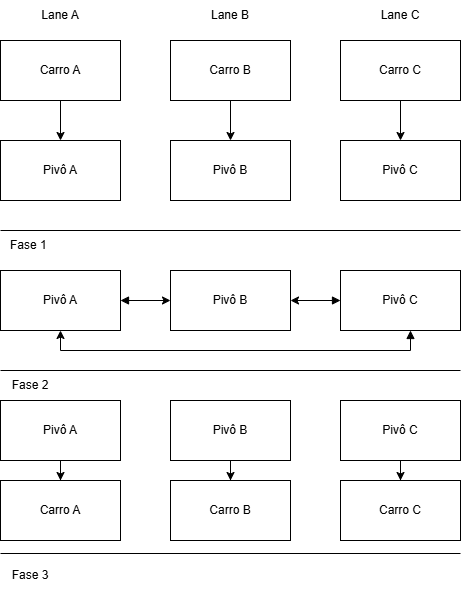
\includegraphics[width=0.85\textwidth]{Chapters/Figures/Arquitertura.drawio.png}
    \caption{Fluxograma das fases do processo de sincronização hierárquica.}
    \label{fig:arq}
\end{figure}

\noindent

\section{Fluxograma e Pseudocódigo da Sincronização Hierárquica}

A Figura~\ref{fig:fluxograma_svsynch} ilustra o fluxo lógico das três fases de sincronização hierárquica no modelo proposto, evidenciando o ciclo. O processo é cíclico e ocorre de forma controlada, garantindo a convergência progressiva do estado global.

\begin{figure}[H]
    \centering
    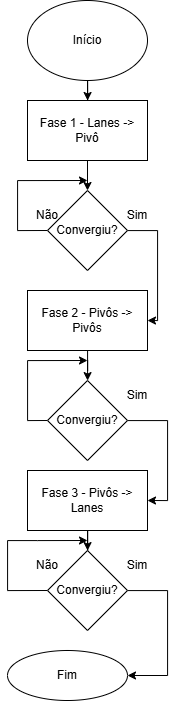
\includegraphics[width=0.2\textwidth]{Chapters/Figures/Fluxograma imp.drawio.png}
    \caption{Fluxograma das fases do processo de sincronização hierárquica.}
    \label{fig:fluxograma_svsynch}
\end{figure}

\newpage
O pseudocódigo simplificado da sincronização hierárquica é apresentado a seguir:

\begin{algorithm}[H]
\caption{Processo de Sincronização Hierárquica.}
\begin{algorithmic}[1]
\State Inicializar conjuntos \textit{Points}, \textit{Pivôs}
\State Definir pivôs com base na proximidade geográfica ao centro da faixa
\State \textbf{Fase 1:} Lanes $\rightarrow$ Pivô
    \Statex \quad Cada veículo envia o seu vetor de estado ao pivô da faixa
    \Statex \quad O pivô agrega e calcula a versão máxima
\State \textbf{Fase 2:} Pivôs $\leftrightarrow$ Pivôs
    \Statex \quad Os pivôs trocam versões agregadas através no centro
    \Statex \quad O pivô com a versão mais alta devolve o vetor global atualizado
\State \textbf{Fase 3:} Pivôs $\rightarrow$ Lanes
    \Statex \quad O estado global é disseminado de volta às faixas
\end{algorithmic}
\end{algorithm}

\section{Critérios para Escolha dos Pivôs}

A seleção dos pivôs é um fator determinante para o desempenho do processo de sincronização. No modelo proposto, a escolha do pivô baseia-se em critérios geográficos, sendo designado como pivô o nó que se encontra mais próximo do centro do cruzamento. Esta escolha visa garantir a menor latência possível na comunicação com os restantes veículos da mesma faixa e principalmente com os pivôs, otimizando, assim, a propagação das mensagens e reduzindo o número de retransmissões necessárias.

\section{Gestão de Mobilidade e Chegada ao Centro}

Durante a simulação, os veículos deslocam-se em direção a um cruzamento urbano. À medida que se aproximam, ocorre uma redistribuição natural das funções de pivô e ponto.  
Os veículos das faixas (lanes) transmitem os seus vetores de estado para o pivô correspondente, enquanto este comunica com os outros nós pivôs.

Quando um ponto atinge a região central, é considerado \textit{chegado ao centro}, sendo incluído na fase de sincronização global. Essa chegada desencadeia uma nova iteração do processo, assegurando que os dados locais são refletidos no estado global antes da dispersão dos veículos.
Em cenários do mundo real, a solução proposta revela-se especialmente útil em situações de paragem temporária, como em cruzamentos controlados por semáforos ou zonas de elevada densidade de tráfego. Nestes momentos, os veículos permanecem estáticos por curtos períodos, proporcionando uma janela ideal para a execução do processo de sincronização hierárquica. Durante esta fase, os nós apresentam uma conectividade mais estável, o que permite aos pivôs recolher e disseminar vetores de estado de forma mais eficiente, reduzindo perdas de pacotes e garantindo a atualização coerente dos dados. Esta abordagem aproveita o comportamento natural do tráfego urbano para otimizar o desempenho do protocolo, melhorando a propagação de informação e a consistência global da rede veicular.
Esta característica torna o modelo proposto particularmente adequado a \gls{ITS} e aplicações cooperativas de segurança, onde a sincronização eficiente entre veículos é essencial para uma tomada de decisão em tempo real.

\section{Estratégia de Sincronização: Determinística vs Assíncrona}

A sincronização hierárquica pode operar segundo dois modos conceptuais:

\begin{itemize}
    \item \textbf{Determinística:} cada fase é executada sequencialmente, apenas iniciando a seguinte após a convergência total da anterior. Esta abordagem garante consistência forte e previsível, sendo ideal para análise experimental.
    \item \textbf{Assíncrona:} as fases sobrepõem-se parcialmente, permitindo que novos dados sejam transmitidos enquanto a sincronização global ainda decorre. Este modo é mais realista em cenários dinâmicos e de alta mobilidade, embora introduza eventual desfasamento temporário de versões.
\end{itemize}

Nas simulações conduzidas, a abordagem determinística foi adotada para permitir a observação clara das fases e o cálculo preciso das métricas de convergência.

\section{Métricas de Avaliação}

As métricas a serem avaliadas no Capítulo~\ref{cha:resultados} permitem quantificar o desempenho do modelo proposto em comparação com o SVSync tradicional.  
A tabela~\ref{tab:metricas_sync} apresenta as principais métricas definidas para análise.

\begin{table}[H]
\centering
\caption{Métricas consideradas para avaliação de desempenho da sincronização hierárquica.}
\label{tab:metricas_sync}
\begin{tabular}{p{4cm} p{10cm}}
\toprule
\textbf{Métrica} & \textbf{Descrição} \\
\midrule
\textbf{Tempo de Convergência} & Intervalo entre o início da sincronização e a obtenção do estado global consistente. \\
\textbf{Número total de Mensagens} & Quantidade total de mensagens de interesse e dados trocadas durante o processo. \\
\textbf{Número de interesses enviados} & Número de interesses que são enviados por todos os nós. \\
\textbf{Número de interesses perdidos} &  Número de interesses que são perdidos no período de sincronização. \\
\textbf{Percentagem de interesses perdidos} & Valor relativo de interesses perididos durante o processo de sincronização. \\
\bottomrule
\end{tabular}
\end{table}

Em conjunto, estas métricas permitem avaliar o impacto da hierarquia proposta na escalabilidade, eficiência e robustez do processo de sincronização.

\section{Limitações e Extensões Futuras}

Embora o modelo proposto apresente vantagens claras em relação ao \gls{SVSync} tradicional, algumas limitações e desafios devem ser considerados:

\begin{itemize}
\item \textbf{Dependência da escolha de pivôs:} A eficiência do protocolo depende da seleção adequada dos pivôs. Em cenários com distribuição irregular de veículos, uma má escolha pode aumentar a latência de convergência. Futuras pesquisas podem explorar algoritmos dinâmicos para selecionar pivôs com base na densidade local de veículos ou na qualidade do link.
\item \textbf{Mudanças rápidas na topologia:} Em situações de tráfego intenso ou manobras inesperadas, veículos podem entrar ou sair das faixas rapidamente, exigindo mecanismos de adaptação para atualizar a hierarquia de forma eficiente.
\item \textbf{Equilíbrio de carga:} Pivôs recebem mensagens de múltiplos veículos, o que pode gerar pontos de concentração de tráfego. Estratégias futuras podem incluir redistribuição temporária de pivôs ou rotas alternativas para mitigar congestionamentos na rede.
\item \textbf{Sincronização assíncrona:} Atualmente, a abordagem determinística garante consistência previsível, mas em cenários altamente dinâmicos, modos assíncronos podem ser explorados para reduzir a latência percebida, mesmo que ocorra desfasamento temporário entre versões.
\end{itemize}

Além disso, o conceito de hierarquia pode ser estendido para ambientes mais complexos:

\begin{itemize}
\item \textbf{Hierarquias multinível:} Em grandes cidades, é possível criar múltiplos níveis de pivôs, onde pivôs locais comunicam-se com pivôs de nível superior, formando uma rede de sincronização capaz de abranger centenas de veículos.
\item \textbf{Integração com sensores urbanos:} Dados provenientes de semáforos, câmeras e sensores de tráfego podem ser incorporados à hierarquia, permitindo que a sincronização veicular também reflita informações do ambiente urbano.
\item \textbf{Adaptação a diferentes padrões de mobilidade:} A estratégia pode ser ajustada para auto-estradas, áreas suburbanas ou ambientes com tráfego misto (veículos autônomos e humanos), mantendo os princípios de agregação de dados e comunicação hierárquica.
\end{itemize}

Em suma, embora o modelo proposto já ofereça ganhos significativos em eficiência e escalabilidade, há espaço para melhorias e adaptações que podem tornar a estratégia ainda mais robusta, flexível e aplicável a cenários urbanos cada vez mais complexos.

\chapter{Implementação}

Este capítulo descreve em detalhe a implementação da solução proposta para a sincronização hierárquica de dados em redes veiculares baseadas em \gls{NDN}. O objetivo é materializar o modelo conceptual apresentado no Capítulo~\ref{chap:estrategia}, avaliando o seu comportamento em diferentes cenários simulados no \texttt{ndnSIM}. A implementação foca-se na integração de uma camada de sincronização hierárquica sobre o mecanismo \gls{SVSync}, permitindo observar o impacto da introdução de pivôs no desempenho global da rede.

\section{Ambiente de Simulação}

A simulação foi realizada utilizando o simulador \texttt{ns-3} com o módulo \texttt{ndnSIM}, o qual fornece suporte nativo para as pilhas de rede \gls{NDN} e para a modelação de estratégias de encaminhamento e cache. O código foi desenvolvido em C++ e recorreu aos módulos principais de mobilidade, aplicações, topologia e análise de métricas do \texttt{ns-3}. A estrutura de ficheiros e dependências segue a organização típica do \texttt{ndnSIM}, assegurando a reprodutibilidade do ambiente.

Os principais módulos incluídos são:

\begin{itemize}
    \item \texttt{core-module}, \texttt{network-module} e \texttt{ndnSIM-module} — para definição da pilha de rede \gls{NDN} e gestão de eventos;
    \item \texttt{mobility-module} — para a simulação da movimentação dos nós;
    \item \texttt{point-to-point-module} e \texttt{point-to-point-layout-module} — para a criação da topologia em grelha e ligações ponto-a-ponto;
    \item \texttt{netanim-module} — para visualização da simulação;
    \item \texttt{applications-module} — para instalação das aplicações de sincronização (SVSync adaptado).
\end{itemize}

Cada nó da rede é configurado com a pilha \gls{NDN} \cite{noauthor_named-datandn-svs_2025} e associado a uma aplicação chamada \textit{chat} baseada em SVSync e que já implementava as premissas do protocolo \cite{shsssc_shssscscenario-svs_2023}, responsável por publicar e sincronizar os dados. A comunicação é realizada através de pacotes \textit{Interest} e \textit{Data}, seguindo as estratégias de encaminhamento \textit{multicast} e \textit{best-route}, definidas no simulador.

\section{Topologia e Parâmetros}

O cenário experimental foi concebido sob a forma de uma grelha bidimensional de nós interligados, com dimensões variáveis consoante o caso de estudo: $5\times5$, $9\times9$, $17\times17$ e $33\times33$.  O número de veículos também aumentava com o aumento da grelha passando de 8 para 16 depois para 32 e por útlimo 64 respetivamente. Esta estrutura permite observar a escalabilidade da solução à medida que o número de veículos aumenta.

\begin{itemize}
    \item A topologia é construída com o auxiliar \texttt{PointToPointGridHelper}, com distância uniforme entre nós e atraso de propagação de $5\,ms$;
    \item A largura de banda das ligações é de $50\,Mbps$;
    \item Cada nó é posicionado fixamente numa coordenada $(x, y)$ e associado a um modelo de mobilidade constante;
    \item Os nós são classificados em duas categorias: \textbf{pontos} (\textit{points}) e \textbf{pivôs} (\textit{pivots}). Os pontos representam veículos comuns, enquanto os pivôs atuam como agregadores e disseminadores de informação na hierarquia;
    \item Cada nó possui uma versão inicial de dados (\texttt{dataVersion}) aleatória, representando estados distintos.
\end{itemize}

A Figura~\ref{fig:grid-exemplo} ilustra o exemplo base de uma grelha $5\times5$, onde se encontram representados os pivôs (nós centrais de cada faixa) e os pontos (nós periféricos que convergem para o centro da topologia).  

A escolha do modelo de mobilidade constante e da topologia em grelha com cruzamento central justifica-se pela necessidade de controlar precisamente o movimento dos nós e as interações entre pivôs e pontos. O modelo de mobilidade constante permite posicionar os veículos em coordenadas fixas, garantindo que os pontos e pivôs se encontrem nos locais corretos para a sincronização hierárquica.  

O cruzamento central na grelha oferece uma margem de manobra temporal e espacial maior permitindo que os pontos se desloquem até o centro sem colisões ou interferências complexase que a sequência das fases de sincronização seja observada de forma clara. Esta configuração facilita o estudo do impacto da hierarquia de pivôs e do tráfego de mensagens, mantendo o cenário suficientemente simples para análise e visualização, mas ainda representativo de situações reais em redes veiculares.

\begin{figure}[H]
    \centering
    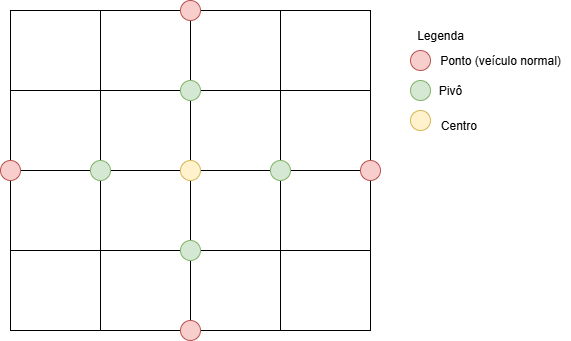
\includegraphics[width=0.65\textwidth]{Chapters/Figures/ExemploCenario.png}
    \caption{Exemplo de cenário proposto com grelha $5\times5$.}
    \label{fig:grid-exemplo}
\end{figure}

Como já referido além do cenário base $5\times5$, foram considerados outros três cenários experimentais com dimensões de grelha maiores: $9\times9$, $17\times17$ e $33\times3$. Em todos os casos, os parâmetros de rede foram mantidos consistentes para permitir comparações diretas:

\begin{itemize}
    \item \textbf{Atraso de propagação das ligações ponto-a-ponto:} $5\,ms$;
    \item \textbf{Largura de banda das ligações:} $50\,Mbps$;
    \item \textbf{Distribuição de pivôs e pontos:} conforme descrito para cada topologia, formando a hierarquia de sincronização;
    \item \textbf{Versões iniciais de dados em cada nó:} aleatórias, representando estados locais distintos.
\end{itemize}

Os valores mencionados correspondem diretamente às configurações utilizadas no código-fonte da simulação, como ilustrado nos seguintes trechos:

\begin{lstlisting}[language=C++]

// Configuração de link P2P
Config::SetDefault("ns3::PointToPointNetDevice::DataRate", StringValue("50Mbps"));
Config::SetDefault("ns3::PointToPointChannel::Delay", StringValue("5ms"));

// Dimensões da grelha
int nRows = 5;
int nCols = 5;
\end{lstlisting}

Além disso, para permitir análise detalhada do desempenho da rede, foram instalados *tracers* do \texttt{ndnSIM}, responsáveis por adquirir métricas de latência e de número de mensagens e interesses trocados.

\begin{lstlisting}[language=C++]
ndn::L3RateTracer::InstallAll("L3RateTracer.txt", Seconds(1.0));
ndn::AppDelayTracer::InstallAll("AppDelayTracer.txt");
\end{lstlisting}

Estas configurações permitem avaliar a escalabilidade da solução, analisando métricas de latência, número total de mensagens trocadas e convergência hierárquica em diferentes densidades de rede, garantindo que os cenários simulados reflitam condições realistas de redes veiculares.

\subsection{Mecanismo de Métricas de Avaliação}

Para analisar o desempenho do modelo proposto, foram definidas métricas específicas que permitem avaliar a eficiência, a fiabilidade e a rapidez do processo de sincronização hierárquica. Estas métricas incidem sobre três aspetos principais:

\begin{itemize}
    \item \textbf{Latência de sincronização:} mede o tempo decorrido desde o envio do primeiro \textit{Interest} até à convergência global da rede. Esta métrica permite avaliar a rapidez com que os dados percorrem a hierarquia de pivôs e alcançam todos os veículos.
    \item \textbf{Taxa de perda de Interesses:} quantifica a percentagem de \textit{Interests} que não obtêm resposta. Esta métrica reflete a fiabilidade da transmissão num ambiente veicular sujeito a falhas e colisões.
    \item \textbf{Número total de mensagens trocadas:} contabiliza todos os pacotes de interesse e de dados transmitidos ao longo do ciclo de sincronização. Esta métrica permite avaliar a eficiência do protocolo hierárquico face a abordagens ponto a ponto tradicionais.
    \item \item \textbf{Número de Interesses Perdidos} contabiliza todos os pacotes de interesse perdidos durante todo o ciclo de sincronização.
    \item \item \textbf{Número total de Interesses enviados:} contabiliza todos os pacotes de interesse enviados ao longo do ciclo de sincronização.
\end{itemize}

\paragraph{Integração com a lógica de sincronização}

Cada nó mantém localmente o seu vetor de estado (\texttt{NodeData}), que é enviado ao pivô da faixa correspondente. Os pivôs agregam os vetores recebidos, determinam a versão mais recente e comunicam no nó central para assegurar coerência global. Após a consolidação da versão global, os pivôs disseminam a informação de volta às faixas, completando o ciclo hierárquico.

Durante este processo, as métricas são calculadas de forma contínua, permitindo obter o volume de mensagens trocadas, a latência observada e a taxa de pacotes perdidos durante a sincronização. Esta abordagem fornece uma visão detalhada do comportamento do protocolo, permitindo identificar pontos críticos oucoportunidades de optimização.

\begin{lstlisting}[language=C++]
void HierarchicalSyncManager::AggregateMetrics(NodeId node)
{
    SyncMetrics[node].interestsSent += node->GetInterestsSent();
    SyncMetrics[node].dataReceived += node->GetDataReceived();
    SyncMetrics[node].latency = node->GetAverageLatency();
}
\end{lstlisting}

Esta função ilustra a recolha centralizada de métricas por pivô, consolidando informação proveniente de múltiplos veículos. Com este mecanismo, é possível analisar o desempenho do modelo proposto, avaliando a escalabilidade do protocolo em diferentes topologias e densidades de nós, como as grelhas $5\times5$, $9\times9$, $17\times17$ e $33\times33$.

A integração destas métricas na simulação permite ainda estudar a robustez do modelo proposto perante mobilidade, fornecendo dados quantitativos essenciais para comparação com abordagens de sincronização tradicionais e para validação do modelo hierárquico.

\section{Estruturas e Módulo de Sincronização Hierárquica}

A implementação da sincronização hierárquica assenta em três componentes fundamentais: a estrutura \texttt{NodeData}, responsável por armazenar o estado individual de cada nó, a estrutura \texttt{SyncMetrics}, utilizada para registar e analisar as métricas de desempenho durante a simulação; e a classe \texttt{Hierarchical\allowbreak Sync\allowbreak Manager}, que orquestra o processo de sincronização em três fases distintas. Estas componentes foram desenvolvidas em C++, totalmente integradas no ambiente \texttt{ndnSIM}, e comunicam com o módulo \gls{SVSync} para manter a coerência dos estados distribuídos.

\subsection{Estrutura \texttt{NodeData}}

A estrutura \texttt{NodeData} representa o estado lógico de cada nó participante na simulação. Cada instância associa um objeto \texttt{Node} do \texttt{ns-3} aos atributos relevantes para o processo de sincronização, incluindo coordenadas na grelha, papéis hierárquicos e versões de dados.

\begin{itemize}
    \item \textbf{Atributos principais:}
    \begin{itemize}
        \item \texttt{node} – apontador para o nó do simulador \texttt{ns-3};
        \item \texttt{row, col} – coordenadas do nó na grelha $N\times N$;
        \item \texttt{name} – identificador textual (e.g., \texttt{Node-2-3});
        \item \texttt{initialDataVersion} e \texttt{dataVersion} – versões inicial e atual dos dados locais, simulando a evolução de informação;
        \item \texttt{isPivot} e \texttt{isPoint} – booleans que distinguem os papéis hierárquicos;
        \item \texttt{hasArrivedAtCenter} – flag usada para verificar a mobilidade dos nós.
    \end{itemize}
    \item \textbf{Função:} abstrair a camada física e topológica do \texttt{ndnSIM}, permitindo manipular o estado lógico dos nós no módulo de sincronização. Esta estrutura serve de base para o cálculo de versões, deteção de convergência e registo de métricas.
\end{itemize}

Cada nó é registado através do método \texttt{RegisterNode()}, o qual inicializa os atributos e atribui uma versão de dados aleatória, garantindo diversidade inicial nos estados.

\subsection{Estrutura \texttt{SyncMetrics}}

A estrutura \texttt{SyncMetrics} implementa um mecanismo simples e eficaz para o registo das métricas de desempenho da sincronização. É composta por variáveis de tempo e funções de registo e análise, conforme apresentado no excerto de código abaixo:

\begin{itemize}
    \item \textbf{Funções principais:}
    \begin{itemize}
        \item \texttt{Start()} – marca o instante de início da sincronização;
        \item \texttt{End()} – regista o instante final e calcula a duração total;
        \item \texttt{WriteFile()} – grava as métricas num ficheiro de texto para posterior análise;
        \item \texttt{RunExternalAnalysis()} – invoca um script Python externo (\texttt{analyze\_tracer.py}) que processa os ficheiros gerados (\texttt{L3RateTracer}, etc.).
    \end{itemize}
\end{itemize}

Este módulo assegura a medição da latência total, e estatísticas de convergência. O registo é iniciado automaticamente quando a primeira fase começa e finalizado após a convergência da última fase.

\subsection{Classe \texttt{HierarchicalSyncManager}}

A classe \texttt{HierarchicalSyncManager} é o núcleo lógico da solução. É responsável por gerir o ciclo de vida da sincronização hierárquica e coordenar as três fases principais que compõem o processo. O gestor é instanciado no início da simulação e mantém listas internas de nós, classificadas em \texttt{points} e \texttt{pivots}, de acordo com a topologia.

\paragraph{Fase 1 – \texttt{Phase1\_LanesToPivots}: Sincronização ascendente.}
Nesta etapa inicial, cada nó da faixa (\textit{point}) envia o seu estado para o respetivo pivô. O objetivo é consolidar as versões locais dos pontos e permitir que o pivô da faixa retenha a versão máxima observada. Em termos práticos, o método verifica no pivô a versão mais alta e atualiza o pivô com essa mesma versão. Esta etapa representa a sincronização ascendente na hierarquia (\textit{bottom-up}).

\paragraph{Fase 2 – \texttt{Phase2\_PivotsInterSync}: Sincronização entre pivôs.}
Uma vez que os pivôs possuem a versão mais recente das respetivas faixas, a segunda fase estabelece a sincronização horizontal entre pivôs. O método calcula a versão máxima entre todos os pivôs e replica-a para cada um deles, garantindo coerência na camada intermédia da hierarquia. Esta fase simboliza a troca de informação entre as faixas e assegura a convergência global antes da disseminação descendente.

\paragraph{Fase 3 – \texttt{Phase3\_PivotsToLanes}: Disseminação descendente.}
A última fase consiste na propagação da versão consolidada dos pivôs de volta aos pontos (\textit{top-down}). Os \textit{points} são atualizados com o valor máximo global, completando assim o ciclo hierárquico de sincronização. Após esta fase, todos os nós, pivôs e  \textit{points} apresentam o mesmo estado de dados, sinalizando a convergência total.

\paragraph{Gestão de fases e verificação de convergência.}
O gestor utiliza um temporizador interno (\texttt{Simulator::\allowbreak Schedule}) para verificar periodicamente se a convergência foi atingida antes de avançar para a fase seguinte. O critério de convergência baseia-se na igualdade das versões entre todos os nós de uma camada. Ao final da terceira fase, o método \texttt{FinishSimulation()} encerra a simulação e aciona o módulo \texttt{SyncMetrics} para registar as métricas.

\subsection{Integração com \gls{SVSync} e ndnSIM}

A solução foi implementada como uma extensão modular sobre o \gls{SVSync}e executada no ambiente \texttt{ndnSIM}. A integração segue dois princípios:

\begin{itemize}
    \item O \gls{SVSync} mantém o estado distribuído dos nós, gerindo a troca de pacotes \texttt{Interest} e \texttt{Data} entre as aplicações \gls{NDN} instaladas. Cada nó executa uma instância de aplicação \gls{SVSync} com prefixo único (por exemplo, \texttt{/2-3}) e parâmetros de publicação (\texttt{PublishDelayMs}) configuráveis.
    \item O módulo \texttt{HierarchicalSyncManager} opera como uma camada de controlo superior, que invoca periodicamente os métodos do \gls{SVSync} para leitura dos vetores de estado (\texttt{GetSvsStateVector()}) e para propagação das versões consolidadas nas fases seguintes.
\end{itemize}

Desta forma, o código mantém a compatibilidade total com o ecossistema \gls{NDN}, reutilizando as bibliotecas de sincronização já existentes no \texttt{ndnSIM}, mas introduzindo um mecanismo hierárquico que reduz a redundância das trocas e melhora a escalabilidade em topologias extensas.

\section{Arquitetura Hierárquica de Sincronização}

A arquitetura implementada baseia-se em três fases de sincronização hierárquica, geridas por um módulo central denominado \textit{Hierarchical Sync Manager}. Este módulo controla a coordenação entre os nós, assegurando a progressão das fases até à convergência total dos estados. O funcionamento segue o modelo conceptual apresentado no Capítulo~3 e é composto pelas seguintes etapas:

\begin{enumerate}
    \item \textbf{Fase 1 – Sincronização dos pontos com os pivôs:} os \textit{points} propagam as suas versões mais recentes para os pivôs da respetiva faixa.
    \item \textbf{Fase 2 – Inter-sincronização entre pivôs:} os pivôs trocam entre si os vetores de estado, garantindo coerência global na camada superior da hierarquia.
    \item \textbf{Fase 3 – Sincronização dos pivôs com os pontos:} após a convergência entre pivôs, estes atualizam os pontos da sua faixa, assegurando a uniformização dos estados em toda a rede.
\end{enumerate}

As três fases são controladas por eventos no simulador, com verificações periódicas de convergência. Cada fase apenas é iniciada quando a anterior atinge estabilidade, isto é, quando todos os nós participantes partilham a mesma versão de dados. O pseudocódigo subjacente encontra-se resumido nas Listas~\ref{lst:phase1} a~\ref{lst:phase3}.

\begin{algorithm}[H]
\caption{Fase 1 – Sincronização dos Pontos para os Pivôs}
\begin{algorithmic}[1]
\State Escrever ``[INST] FASE 1 - Pontos enviam as versões mais recentes aos pivôs''
\State $maxVersaoPontos \gets -1$
\For{cada ponto em \textit{points}}
    \If{ponto não é pivô}
        \If{$ponto.dataVersion > maxVersaoPontos$}
            \State $maxVersaoPontos \gets ponto.dataVersion$
        \EndIf
    \EndIf
\EndFor
\For{cada pivô em \textit{pivots}}
    \If{$pivô.dataVersion < maxVersaoPontos$}
        \State $pivô.dataVersion \gets maxVersaoPontos$
    \EndIf
\EndFor
\end{algorithmic}
\end{algorithm}

\begin{algorithm}[H]
\caption{Fase 2 – Inter-sincronização entre Pivôs}
\begin{algorithmic}[1]
\State Escrever ``[INST] FASE 2 - Pivôs trocam versões entre si''
\State $maxVersaoPivos \gets -1$
\For{cada pivô em \textit{pivots}}
    \If{$pivô.dataVersion > maxVersaoPivos$}
        \State $maxVersaoPivos \gets pivô.dataVersion$
    \EndIf
\EndFor
\For{cada pivô em \textit{pivots}}
    \State $pivô.dataVersion \gets maxVersaoPivos$
\EndFor
\end{algorithmic}
\end{algorithm}

\begin{algorithm}[H]
\caption{Fase 3 – Disseminação dos Pivôs para os Pontos}
\begin{algorithmic}[1]
\State Escrever ``[INST] FASE 3 - Pivôs actualizam todos os pontos''
\State $maxVersaoPivos \gets -1$
\For{cada pivô em \textit{pivots}}
    \If{$pivô.dataVersion > maxVersaoPivos$}
        \State $maxVersaoPivos \gets pivô.dataVersion$
    \EndIf
\EndFor
\For{cada ponto em \textit{points}}
    \State $ponto.dataVersion \gets maxVersaoPivos$
\EndFor
\end{algorithmic}
\end{algorithm}

Após a execução das três fases, todos os nósn alcançam a mesma versão final dos dados, simbolizando a convergência global do estado da rede.

\section{Execução e Métricas de Avaliação}

A simulação é executada em diferentes topologias ($5\times5$, $9\times9$, $17\times17$ e $33\times33$), permitindo observar o comportamento do sistema em escalas crescentes de densidade veicular. 

O sistema regista, então, automaticamente as seguintes métricas, Latência de Sincronização, Taxa de perda de Interesses, Número total de mensagens trocadas, Número de Interesses Perdidos e Número total de Interesses enviados.

Os resultados são gravados em ficheiros de texto e posteriormente analisados por um script externo em \texttt{Python}, que produz os gráficos apresentados no Capítulo~5.


\section{Script de Análise dos Resultados}

Para processar os resultados gerados pelas simulações no \textit{ndnSIM}, foi desenvolvido um script em Python responsável por extrair e calcular métricas de desempenho a partir dos ficheiros de traço \textit{AppDelayTracer.txt} e \textit{L3RateTracer.txt}. 

O objetivo deste script é automatizar a leitura dos ficheiros de saída, filtrar os dados relevantes dentro de um intervalo de tempo específico e calcular estatísticas fundamentais, como latência, número de pacotes transmitidos, recebidos e perdidos durante o processo de sincronização.

O código apresentado na Listagem~\ref{lst:python_analysis} contém as 2 funções principais:

\begin{itemize}
    \item \texttt{analyze\_app\_delay\_tracer()}: lê o ficheiro \texttt{AppDelayTracer.txt}
    \item \texttt{analyze\_l3\_tracer()}: processa o \texttt{L3RateTracer.txt} para contabilizar pacotes \textit{Interest}, \textit{Data} e \textit{Nack}, permitindo estimar a perda de pacotes.
\end{itemize}

O programa principal recebe como argumentos o tempo inicial e final da análise, correspondendo ao período efetivo de sincronização, e apresenta um resumo das métricas calculadas no terminal.

\begin{lstlisting}[language=Python, caption={Script de análise de resultados da simulação}, label={lst:python_analysis}]
avg_lat, min_lat, max_lat = analyze_app_delay_tracer(start_time, end_time)
tx_interests, rx_interests, tx_data, rx_data, tx_nacks = analyze_l3_tracer(start_time, end_time)

interest_loss = tx_interests - rx_interests
total_sync_packets = tx_interests + rx_interests + tx_data + rx_data
\end{lstlisting}

Este script foi utilizado em todas asnsimulações para garantir consistência no cálculo das métricas e facilitar a geração de gráficos de desempenho apresentados no capítulo seguinte.

\section{Fluxo Lógico da Sincronização}

A Figura~\ref{fig:fluxograma-codigo} sintetiza a sequência lógica de operações da simulação, desde a configuração inicial dos nós até à fase de convergência. Mostra assim de forma clara todos os passos que a simulação percorre.

\begin{figure}[H]
    \centering
    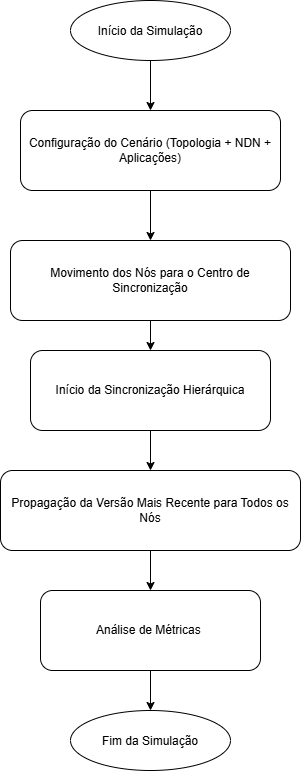
\includegraphics[width=0.3\textwidth]{Chapters/Figures/Fluxograma.png}
    \caption{Fluxograma do funcionamento da sincronização hierárquica.}
    \label{fig:fluxograma-codigo}
\end{figure}

\section{Síntese}

A implementação desenvolvida demonstra a viabilidade da abordagem hierárquica com pivôs no contexto das redes \gls{V-NDN}. Através da simulação no \texttt{ndnSIM}, foi possível observar a convergência eficiente de estados num ambiente dinâmico e distribuído, preservando a compatibilidade com o protocolo \gls{SVSync}. No capítulos seguinte são apresentados os resultados quantitativos obtidos e a análise comparativa entre as diferentes topologias.

%%%%%%%%%%%%%%%%%%%%%%%%%%%%%%%%%%%%%%%%%%%%%%%%%%
\chapter{Resultados}
\label{cha:resultados}
%%%%%%%%%%%%%%%%%%%%%%%%%%%%%%%%%%%%%%%%%%%%%%%%%%

\section{Introdução}

Este capítulo apresenta e discute os resultados experimentais obtidos com a implementação da solução de sincronização hierárquica, comparando-a com o modelo tradicional sem hierarquia. O principal objetivo desta avaliação é demonstrar a eficácia da abordagem proposta quanto à redução da latência, tráfego de mensagens e perdas de pacotes avaliando igualmente a sua \textbf{escalabilidade}, \textbf{robustez} e \textbf{eficiência de recursos}.

Os testes foram conduzidos no simulador ndnSIM, utilizando diferentes topologias em grelha, com número crescente de nós, representando veículos em movimento. As métricas de desempenho foram recolhidas a partir do ficheiro de análise (\texttt{L3RateTracer}) permitindo comparar, de forma quantitativa, as duas abordagens.

%%%%%%%%%%%%%%%%%%%%%%%%%%%%%%%%%%%%%%%%%%%%%%%%%%
\section{Descrição do Cenário Experimental}
%%%%%%%%%%%%%%%%%%%%%%%%%%%%%%%%%%%%%%%%%%%%%%%%%%

A simulação foi concebida para avaliar o comportamento do modelo proposto em topologias de 5×5, 9×9, 17×17 e 33×33 nós,ou seja, aumento o número de nós (veículos) de 8 para 16 para 32 e 64, respetivamente, de modo a representar diferentes densidades de veículos.  
Em todas as configurações, manteve-se a estrutura hierárquica proposta no Capítulo \ref{chap:estrategia}, com pivôs posicionados nos eixos mais próximos do centro da grelha e um nó central onde ocorre o processo.

Cada nó executa a aplicação chat do NDN-SVS \cite{shsssc_shssscscenario-svs_2023}, responsável pela publicação periódica de interesses e atualização dos estados locais. As comunicações entre nós foram configuradas com ligações ponto-a-ponto.

Os nós seguem um modelo de mobilidade constante, em que os pontos se deslocam gradualmente em direção ao centro da grelha, reproduzindo um cenário realista de convergência veicular.

\begin{table}[h!]
\centering
\caption{Parâmetros de simulação}
\begin{tabular}{ll}
\toprule
\textbf{Parâmetro} & \textbf{Valor} \\ 
\midrule
Simulador & ndnSIM (NS-3) \\
Topologias & 5×5, 9×9, 17×17, 33×33 \\
Largura de banda dos links & 50 Mbps \\
Atraso de propagação & 5 ms \\
Intervalo de publicação & 0,8 s (rápido) / 1,5 s (lento) \\
Métricas analisadas & Mensagens totais, perdas e tempo de sincronização \\ 
\bottomrule
\end{tabular}
\end{table}

Esta configuração assegura condições comparáveis entre cenários e permite observar o impacto da hierarquia no desempenho global do sistema.

%%%%%%%%%%%%%%%%%%%%%%%%%%%%%%%%%%%%%%%%%%%%%%%%%%
\section{Análise Comparativa por Métrica}

\subsection{Latência}

A Figura \ref{fig:lnh} mostra a evolução da latência em função do número de nós.  
Enquanto a abordagem sem hierarquia apresenta um aumento grande com a dimensão da rede, a solução hierárquica mantém uma tendência linear e estável, resultado direto da redução de saltos de sincronização e da eliminação de interesses redundantes.

\begin{figure}[h!]
\centering
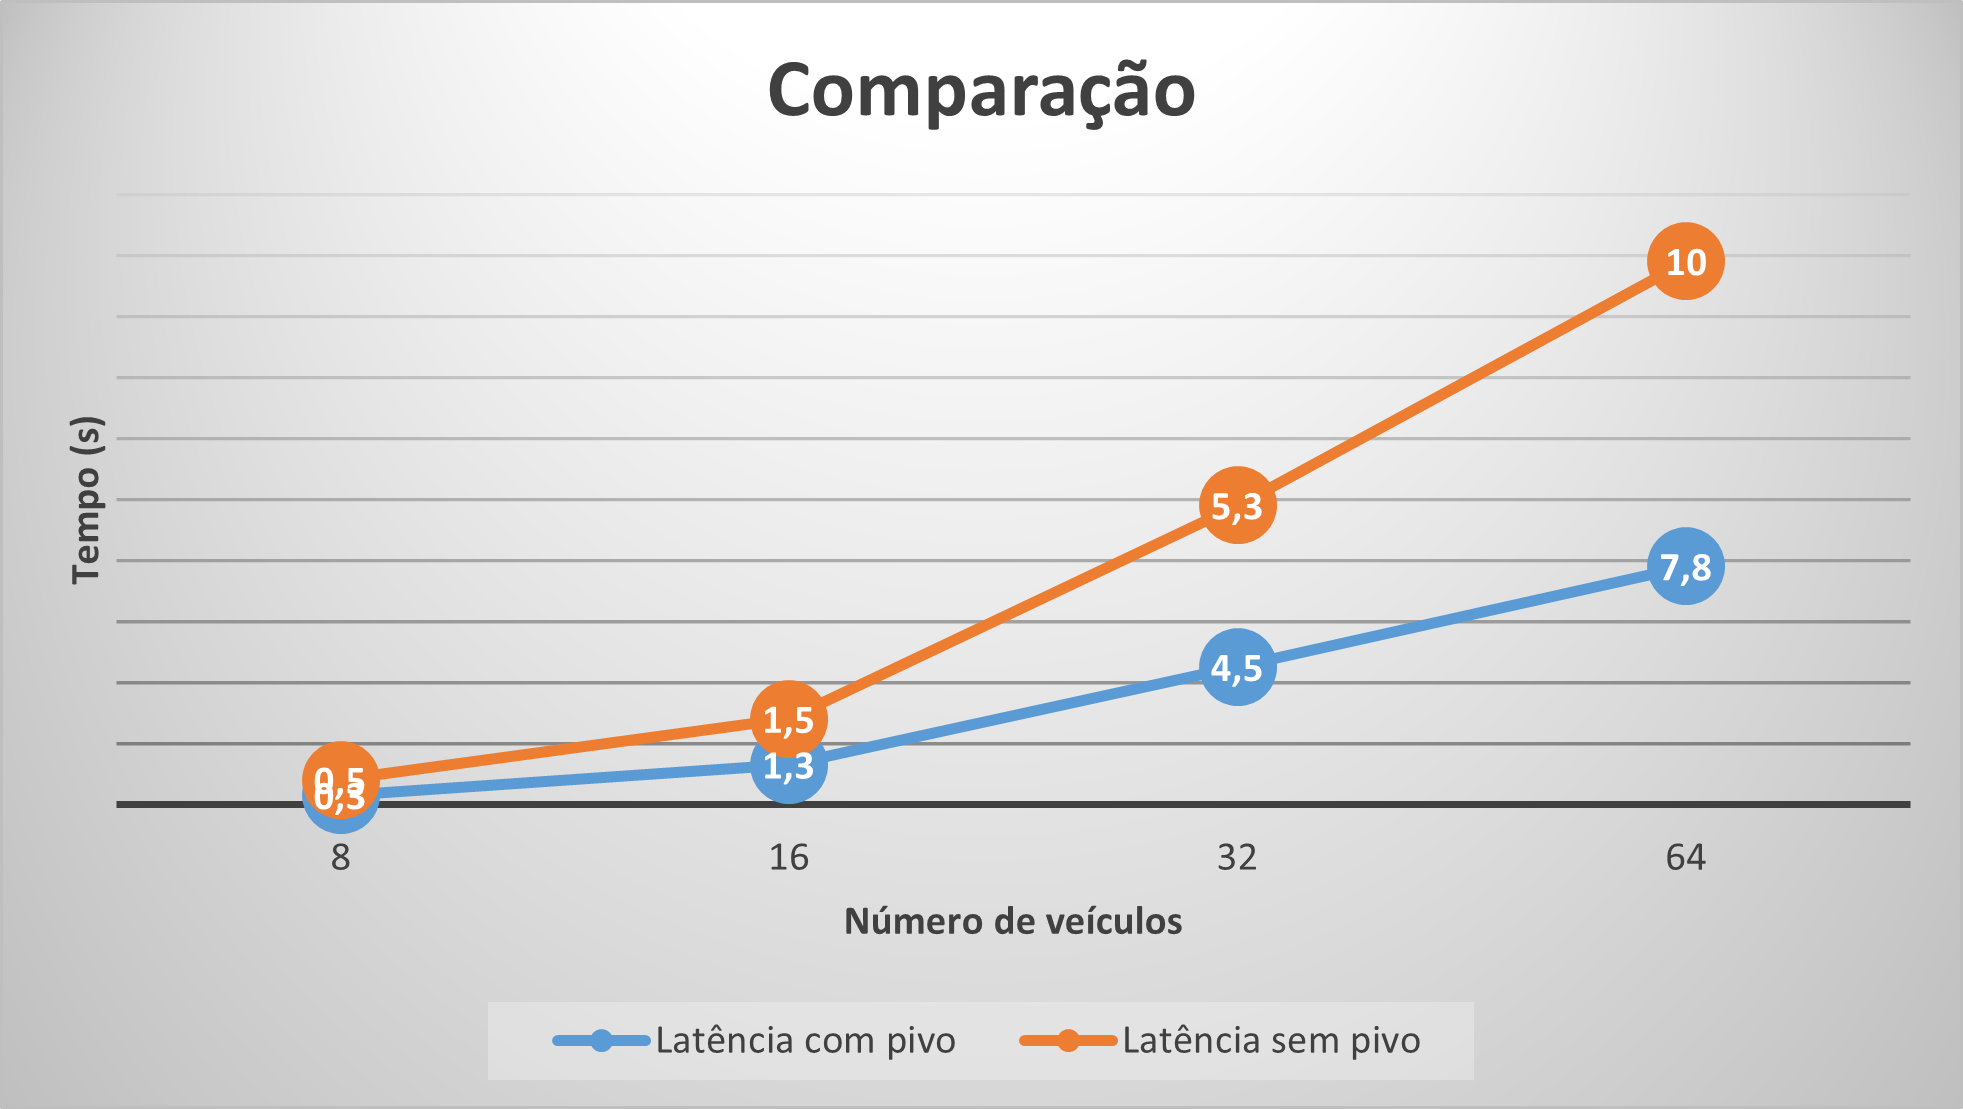
\includegraphics[width=0.9\textwidth]{Chapters/Figures/LatenciaNH.png}
\caption{Comparação da latência entre as soluções sem hierarquia e hierárquica.}
\label{fig:lnh}
\end{figure}
A Tabela~\ref{tab:latencia_pivo} apresenta a comparação entre os valores de latência obtidos com e sem a utilização do pivô, para diferentes números de carros. Observa-se que, em todos os casos, a introdução do pivô resultou numa redução da latência. 

Para um número reduzido de carros (8 veículos), a diminuição é de aproximadamente 40\%, evidenciando um impacto bastante significativo. À medida que o número de carros aumenta, a diferença relativa tende a estabilizar entre 13\% e 22\%, o que demonstra que o mecanismo de pivô continua a ser vantajoso, mesmo em cenários mais exigentes em termos de carga.

Estes resultados indicam que a utilização do pivô contribui para uma melhoria consistente do desempenho do sistema, reduzindo o tempo de resposta global e aumentando a eficiência da comunicação entre veículos.

\begin{table}[H]
\centering
\caption{Comparação da latência com e sem pivô em função do número de carros.}
\label{tab:latencia_pivo}
\begin{tabular}{cccc}
\toprule
\textbf{Nº de carros} & \textbf{Latência com pivô (s)} & \textbf{Latência sem pivô (s)} & \textbf{Diferença relativa (\%)} \\ 
\midrule
8  & 0.3 & 0.5 & -40.0 \\
16 & 1.3 & 1.5 & -13.3 \\
32 & 4.5 & 5.3 & -15.1 \\
64 & 7.8 & 10.0 & -22.0 \\
\bottomrule
\end{tabular}
\end{table}

\subsection{Número Total de Mensagens}

A Figura \ref{fig:ITNH} ilustra a quantidade total de mensagens trocadas em ambas as abordagens.  
O modelo sem hierarquia gera tráfego exponencial com o crescimento da rede, resultando em sobrecarga da \gls{PIT} e aumento do risco de colisões.  
Já o modelo proposto restringe a propagação de interesses a cada camada de pivôs, limitando o tráfego global.

\begin{figure}[h!]
\centering
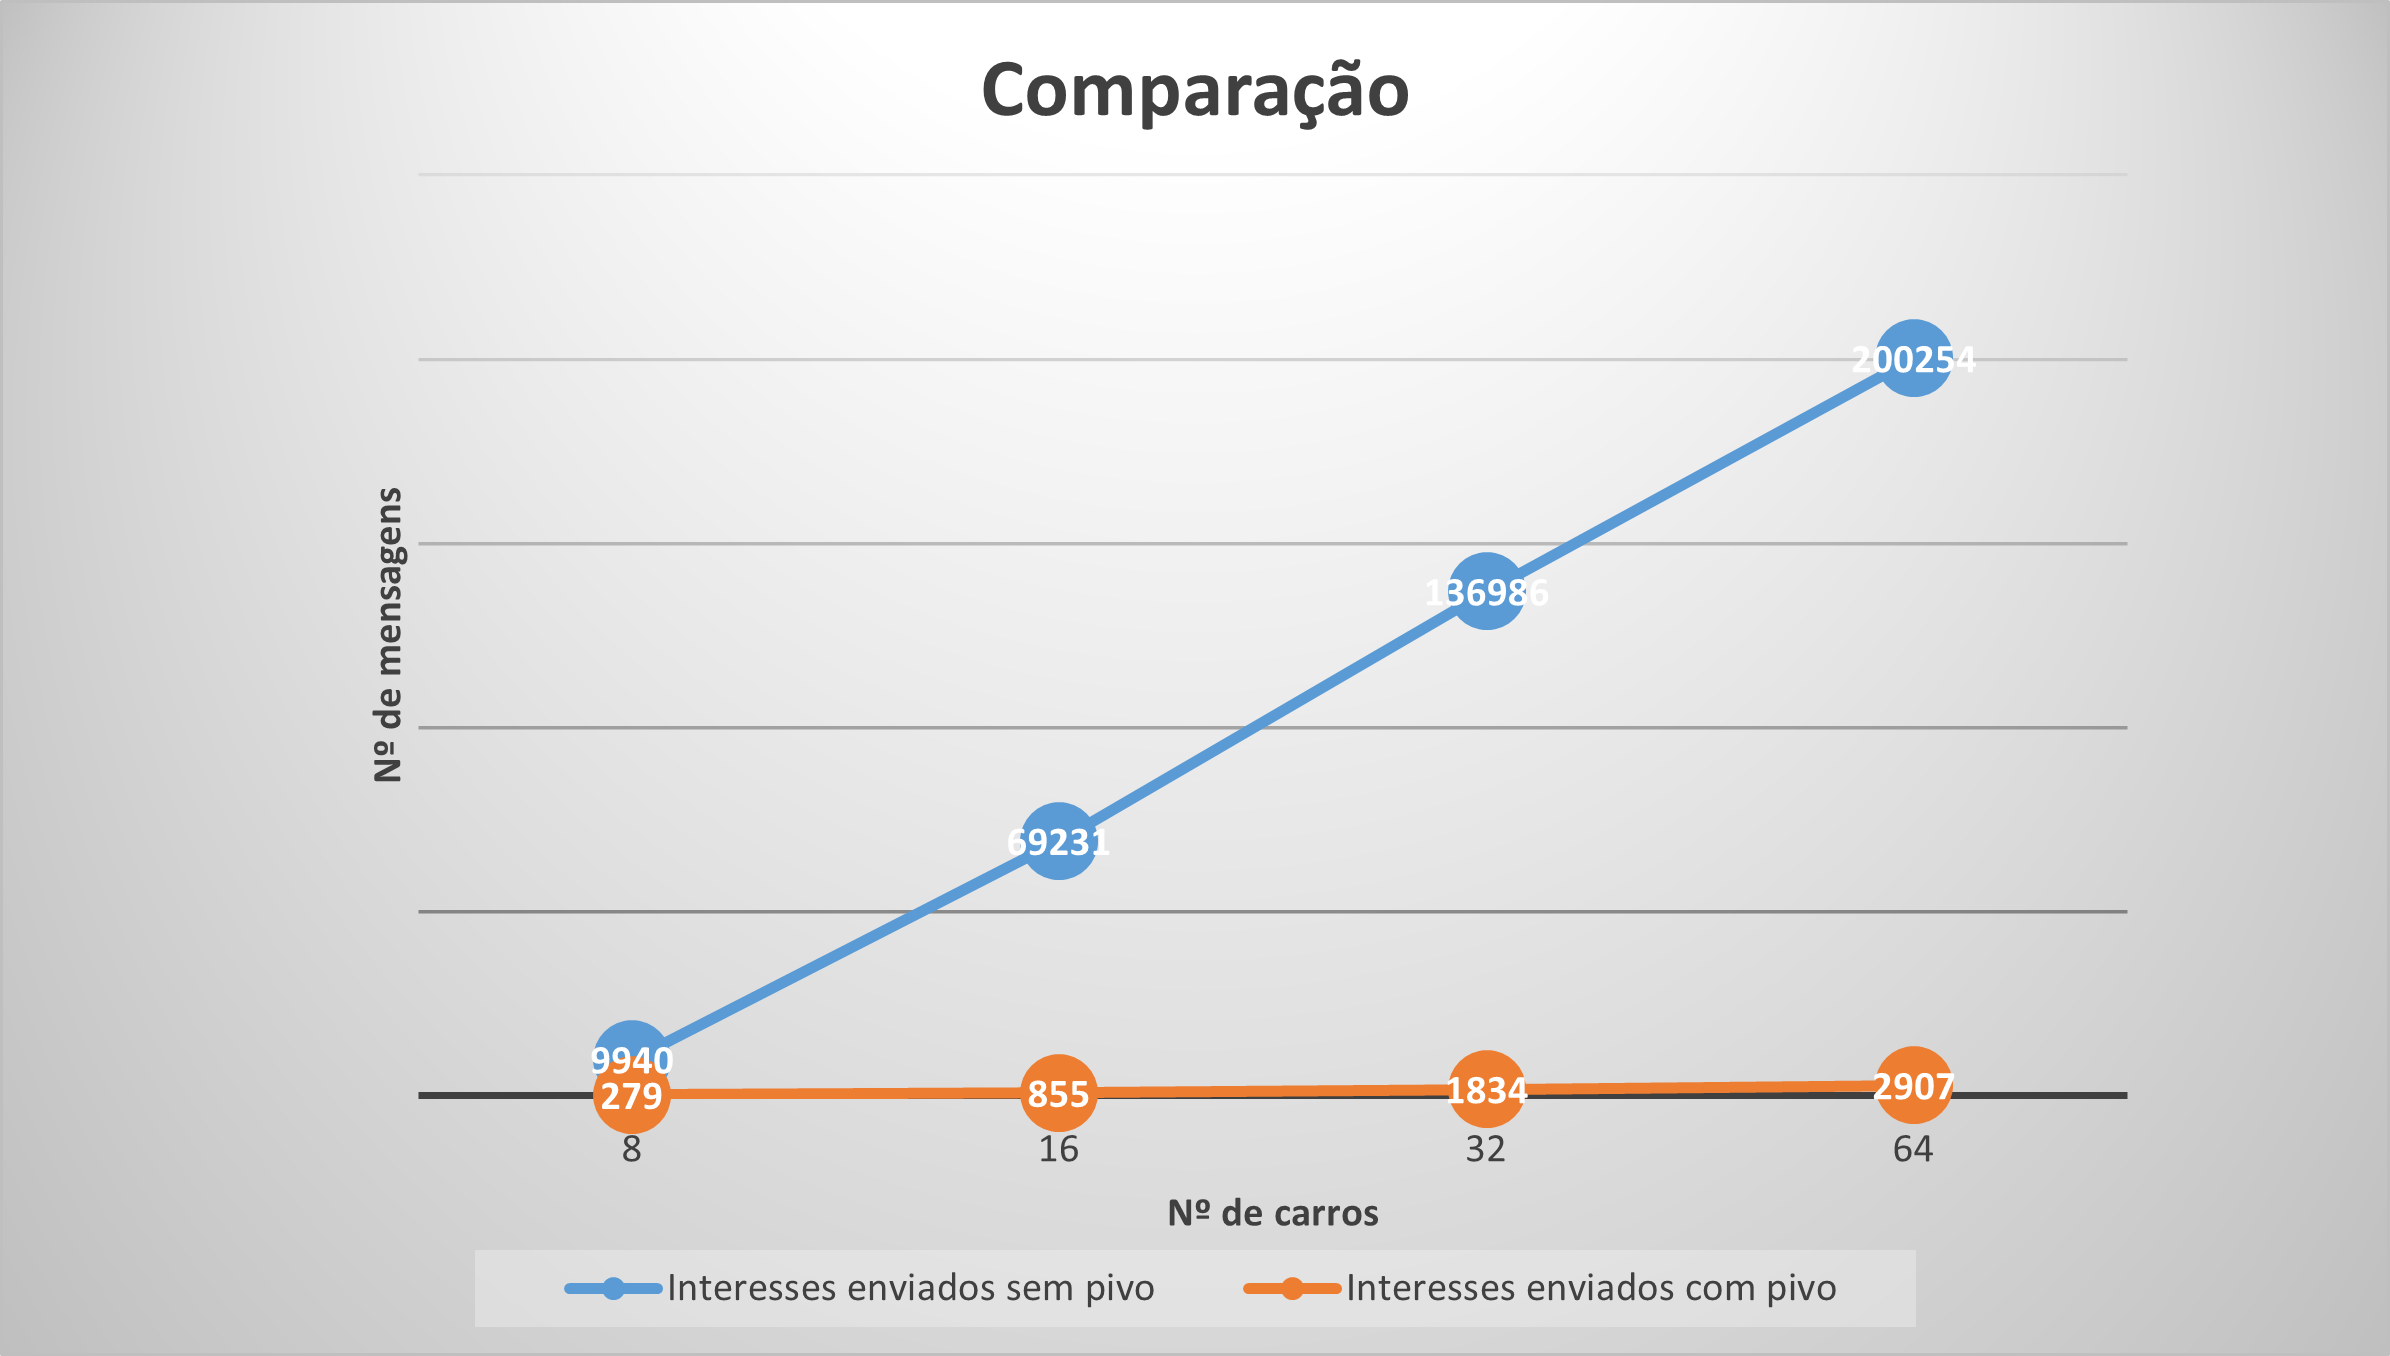
\includegraphics[width=0.9\textwidth]{Chapters/Figures/Interessesehn.png}
\caption{Número total de interesses trocados nas soluções sem e com hierarquia.}
\label{fig:ITNH}
\end{figure}

A Tabela~\ref{tab:mensagens_pivo} apresenta a comparação do número total de mensagens trocadas no sistema, com e sem a utilização do pivô, para diferentes números de carros. Observa-se uma redução extremamente significativa no volume de mensagens quando é utilizada a abordagem hierárquica com pivô.
\begin{table}[H]
\centering
\caption{Comparação do número total de mensagens trocadas com e sem pivô em função do número de carros.}
\label{tab:mensagens_pivo}
\begin{tabular}{cccc}
\toprule
\textbf{Nº de carros} & \textbf{Mensagens com pivô} & \textbf{Mensagens sem pivô} & \textbf{Diferença relativa (\%)} \\ 
\midrule
8  & 348   & 12821  & -97.3 \\
16 & 1071  & 97916  & -98.9 \\
32 & 2406  & 186438 & -98.7 \\
64 & 3795  & 291987 & -98.7 \\
\bottomrule
\end{tabular}
\end{table}

Para 8 veículos, o número total de mensagens diminui de 12821 para apenas 348, o que corresponde a uma redução de cerca de 97\%. À medida que o número de veículos aumenta, esta redução mantém-se acima dos 98\%, evidenciando a excelente escalabilidade e a eficiência no controlo de congestionamento da solução hierárquica.

Este comportamento confirma que a utilização do pivô permite concentrar e organizar as comunicações de forma mais eficiente, evitando a a troca de mensagens redundantes e reduzindo de forma drástica o tráfego de rede. Assim, o sistema torna-se mais escalável e adequado para cenários com elevado número de veículos. Podemos ainda dizer que temos valores muito altos pois estão a ser enviados interesses em espaços temporais muito curtos, o que gera muitas colisões e perdas por processamento de mensagens, não invalidando, assim, o modelo proposto.

\subsection{Percentagem de Perdas}

As perdas de interesses devem-se principalmente a colisões e ao envio simultâneo de múltiplos pedidos.  
Como ilustrado nas Figuras \ref{fig:IPPH} e \ref{fig:IPPP}.

\begin{figure}[h!]
\centering
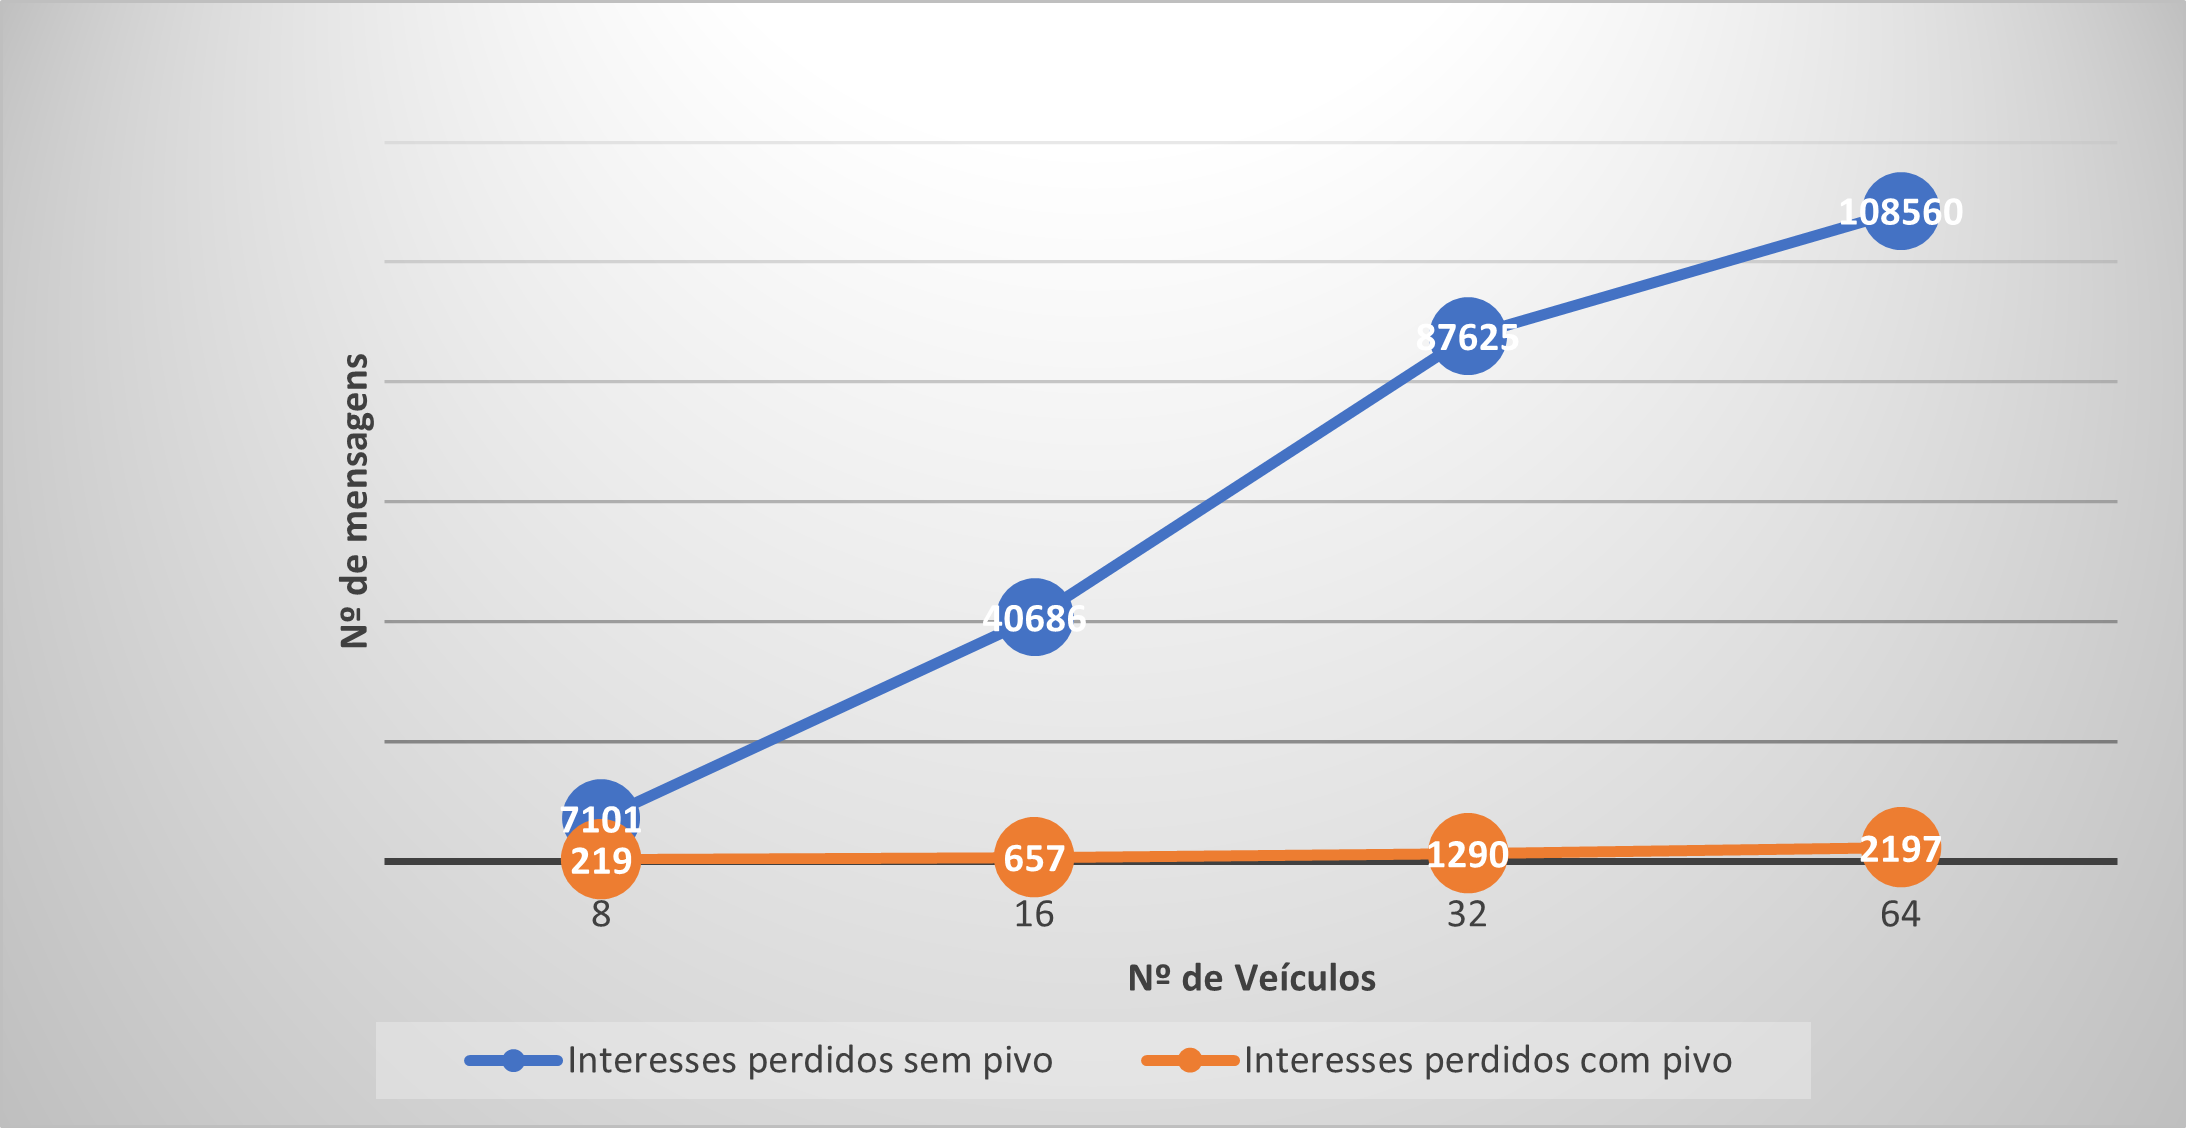
\includegraphics[width=0.9\textwidth]{Chapters/Figures/Interessesphn.png}
\caption{Interesses perdidos nas abordagens sem e com hierarquia.}
\label{fig:IPPH}
\end{figure}

A Tabela~\ref{tab:interesses_perdidos} apresenta o número de interesses perdidos, bem como a percentagem relativa de perdas, comparando a solução com e sem pivô. Verifica-se que a abordagem hierárquica conduz a uma redução significativa do número 
absoluto de interesses perdidos em todos os cenários testados.

\begin{figure}[h!]
\centering
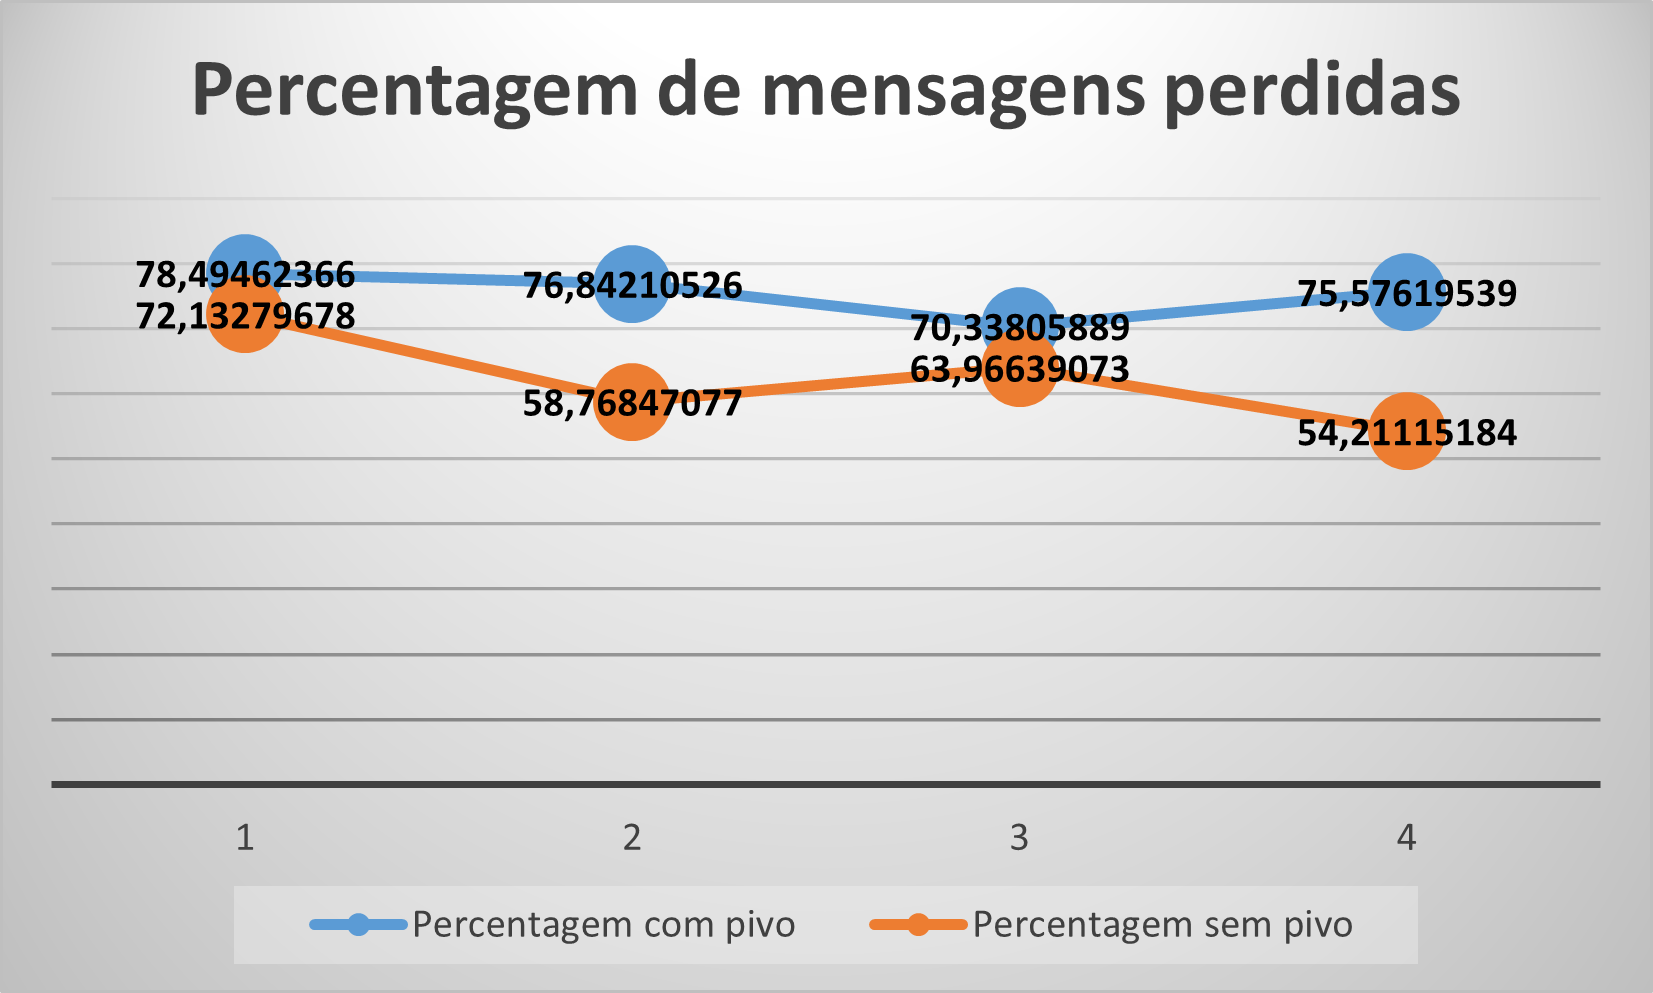
\includegraphics[width=0.9\textwidth]{Chapters/Figures/InteressesPP.png}
\caption{Percentagem de interesses perdidos em função do número de nós.}
\label{fig:IPPP}
\end{figure}

Para 8 veículos, a  solução sem pivô regista 7101 interesses perdidos, enquanto a solução com pivô apresenta apenas 219, representando uma melhoria substancial. Esta tendência mantém-se à medida que o número de carros aumenta, com reduções superiores a 95\% no total de interesses perdidos.  
Em termos percentuais, a taxa de sucesso (interesses bem processados) é consistentemente mais elevada quando se utiliza o pivô, situando-se entre 70\% e 78\%, face a valores entre 54\% e 72\% no caso sem pivô.

A Tabela~\ref{tab:interesses_enviados} e a Figura~\ref{fig:interesses_enviados} ilustram o impacto da utilização do pivô no número total de interesses enviados e na percentagem de sucesso.  
Observa-se uma redução muito significativa no volume de mensagens quando é utilizada a abordagem hierárquica, acompanhada por uma taxa de sucesso mais elevada e mais estável, mesmo à medida que o número de veículos aumenta.
Por exemplo, com 64 veículos, o número de interesses enviados cai de 200~254 para apenas 2907, o que representa uma diminuição de cerca de 98.5\%. Por exemplo, no cenário com 64 carros, o número de interesses enviados diminui de 200~254 (sem pivô) para apenas 2907 (com pivô), o que representa uma redução superior a 98\%. Em simultâneo, a percentagem de sucesso mantém-se acima dos 75\%, enquanto que na configuração sem pivô desce para cerca de 54\%.  

\begin{table}[H]
\centering
\caption{Comparação do número total de interesses enviados e respetivas percentagens de sucesso, com e sem pivô.}
\label{tab:interesses_enviados}
\begin{tabular}{ccccc}
\toprule
Nº de carros & Interesses enviados com pivô & Interesses enviados sem pivô & \% com pivô & \% sem pivô \\ 
\midrule
8  & 279  & 9940   & 78.5 & 72.1 \\
16 & 855  & 69231  & 76.8 & 58.8 \\
32 & 1834 & 136986 & 70.3 & 64.0 \\
64 & 2907 & 200254 & 75.6 & 54.2 \\
\bottomrule
\end{tabular}
\end{table}

\begin{table}[H]
\centering
\caption{Comparação do número de interesses perdidos com e sem pivô.}
\label{tab:interesses_perdidos}
\begin{tabular}{ccccc}
\toprule
Nº de carros & Interesses perdidos com pivô & Interesses perdidos sem pivô & \% com pivô & \% sem pivô \\ 
\midrule
8  & 219  & 7101   & 78.5 & 72.1 \\
16 & 657  & 40686  & 76.8 & 58.8 \\
32 & 1290 & 87625  & 70.3 & 64.0 \\
64 & 2197 & 108560 & 75.6 & 54.2 \\
\bottomrule
\end{tabular}
\end{table}

\begin{figure}[H]
\centering

\includegraphics[width=0.8\textwidth]{Interessesehn.png}
\caption{Evolução do número de interesses enviados com e sem pivô em função do número de carros.}
\label{fig:interesses_enviados}
\end{figure}

Estes resultados confirmam que a solução hierárquica com pivô não só reduz drasticamente o tráfego de rede, como também melhora a eficiência e a fiabilidade do processo de disseminação de interesses, contribuindo para um comportamento mais escalável e controlado do sistema.

\section{Taxa da rede}

A Tabela~\ref{tab:taxa_rede} apresenta a eficiência da rede, calculada como a razão entre o número de interesses entregues com sucesso e o total de interesses enviados. 
\begin{table}[H]
\centering
\caption{Taxa da rede (eficiência de entrega de interesses) com e sem pivô.}
\label{tab:taxa_rede}
\resizebox{\textwidth}{!}{%
\begin{tabular}{ccccccc}
\toprule
Nº de carros & Enviados c/ pivô & Perdidos c/ pivô & Taxa c/ pivô (\%) & Enviados s/ pivô & Perdidos s/ pivô & Taxa s/ pivô (\%) \\ 
\midrule
8  & 279  & 219  & 21.5 & 9940   & 7101   & 28.6 \\
16 & 855  & 657  & 23.1 & 69231  & 40686  & 41.2 \\
32 & 1834 & 1290 & 29.6 & 136986 & 87625  & 36.1 \\
64 & 2907 & 2197 & 24.4 & 200254 & 108560 & 45.8 \\
\bottomrule
\end{tabular}%
}
\end{table}

Observa-se que a taxa percentual de rede é ligeiramente inferior na configuração com pivô, variando entre 21\% e 30\%, em comparação com valores entre 28\% e 46\% na abordagem sem pivô. 

No entanto, esta diferença deve ser interpretada em conjunto com o volume total de mensagens. 
Apesar de uma menor taxa percentual, o número absoluto de mensagens trocadas e de interesses perdidos é várias ordens de grandeza inferior na abordagem hierárquica, o que indica uma utilização muito mais eficiente dos recursos da rede. 
Em termos globais, a estratégia com pivô demonstra um comportamento mais estável e controlado, reduzindo a sobrecarga de comunicação e assegurando uma sincronização eficaz mesmo em cenários com elevado número de veículos.

%%%%%%%%%%%%%%%%%%%%%%%%%%%%%%%%%%%%%%%%%%%%%%%%%%

%%%%%%%%%%%%%%%%%%%%%%%%%%%%%%%%%%%%%%%%%%%%%%%%%%

\section{Análise de Escalabilidade}

A escalabilidade é um fator determinante na viabilidade de sistemas distribuídos.  
Nos testes realizados, observou-se que o crescimento da rede não provoca uma degradação linear das métricas no modelo hierárquico.  
Enquanto a abordagem plana apresenta aumento exponencial da latência e do tráfego, o modelo proposto mantém uma evolução quase linear.

Nas grelhas menores (5×5), as diferenças são reduzidas, dado o baixo número de interações. No entanto, com o aumento do número de veículos, a abordagem sem hierarquia torna-se inviável devido à sobrecarga, enquanto o modelo hierárquico conserva a estabilidade e previsibilidade.  
Este comportamento comprova a capacidade de escalabilidade do modelo proposto para redes de larga escala.

%%%%%%%%%%%%%%%%%%%%%%%%%%%%%%%%%%%%%%%%%%%%%%%%%%
%%%%%%%%%%%%%%%%%%%%%%%%%%%%%%%%%%%%%%%%%%%%%%%%%%
\section{Limitações e Perspetivas Futuras}

Apesar dos resultados positivos, a abordagem proposta apresenta algumas limitações.  
Em cenários extremamente grandes, a distância entre pivôs pode introduzir atrasos adicionais na Fase 2 da sincronização.  
Além disso, o modelo assume uma estrutura de rede relativamente estática, o que não reflete plenamente o comportamento de veículos em movimento contínuo.

Como evolução futura, propõe-se:
\begin{itemize}
    \item Implementar algoritmos de eleição dinâmica de pivôs, adaptativos à mobilidade e densidade da rede;
    \item Integrar mecanismos de ajuste automático do intervalo de publicação, com base na carga de tráfego observada;
    \item Avaliar o o modelo em ambientes urbanos reais, com dados de mobilidade obtidos de simuladores como SUMO ou de GPS.
\end{itemize}

%%%%%%%%%%%%%%%%%%%%%%%%%%%%%%%%%%%%%%%%%%%%%%%%%%
\section{Síntese Final}

De forma resumida, o modelo proposto apresenta ganhos expressivos em todas as métricas avaliadas. A abordagem hierárquica demonstrou:

\begin{itemize}
    \item Redução drástica do tráfego de mensagens, com diminuição superior a 98\% no número total de mensagens e interesses enviados em comparação com a abordagem sem pivô;
    \item Latências significativamente menores, com melhoria de até 40\% em cenários com poucos veículos e redução consistente entre 13\% e 22\% em cenários mais carregados;
    \item Maior fiabilidade na entrega de interesses, com taxa de sucesso mantida acima de 70\%, face a valores entre 54\% e 64\% sem pivô;
    \item Menor número de interesses perdidos, reforçando a capacidade de resistência a congestionamentos e de escalabilidade do sistema.
\end{itemize}

Em conclusão, os resultados confirmam que o modelo proposto constitui uma solução eficiente, escalável e robusta para a sincronização de dados em redes veiculares \gls{NDN}. A sua capacidade de reduzir drasticamente o tráfego, manter baixas latências e garantir elevada fiabilidade valida a aplicabilidade da proposta em cenários cooperativos e de elevada mobilidade, fundamentais para a próxima geração de sistemas de transporte inteligentes.


\chapter{Conclusão e Trabalho Futuro}

\section{Síntese Geral}
O presente trabalho teve como objetivo propor e avaliar uma estratégia hierárquica de sincronização de dados em redes veiculares baseadas no paradigma \gls{NDN}. A abordagem desenvolvida, suportada pelo protocolo \gls{SVSync}, introduz a utilização de nós \textit{pivôs} como elementos de agregação e disseminação de informação, com o intuito de reduzir a sobrecarga de mensagens e a latência de sincronização em cenários com elevada densidade veicular.

A implementação foi realizada no \texttt{ndnSIM}, considerando cenários em grelha com tamanhos 5x5, 9x9, 17x17 e 33x33, representando interseções urbanas com múltiplas faixas. O código define três fases de sincronização distintas, \textit{Lanes to Pivots}, \textit{Pivots Inter-Sync} e \textit{Pivots to Lanes} recolhendo métricas como a duração total do processo de sincronização, número de mensagens trocadas e taxa de perda de \textit{Interests}.

Os resultados demonstram que a abordagem hierárquica apresenta vantagens significativas relativamente à solução tradicional (sem pivôs). Em particular:
\begin{itemize}
\item a latência de sincronização é significativamente reduzida e mantém-se estável mesmo com o aumento do número de veículos e do tamanho da rede;
\item o número total de mensagens trocadas diminui substancialmente, evitando a sobrecarga observada em abordagens planas;
\item a taxa de perda de \textit{Interests} mantém-se dentro de valores aceitáveis, comprovando a robustez do modelo proposto.
\end{itemize}

Estes resultados confirmam que a hierarquização da sincronização, com eleição de pivôs por faixa de tráfego, permite melhorar a escalabilidade e a eficiência da disseminação de dados em ambientes densos e dinâmicos, típicos de redes veiculares.

\section{Limitações Identificadas}
Apesar do desempenho positivo, a solução proposta apresenta algumas limitações importantes:
\begin{itemize}
\item \textbf{Mobilidade e conectividade intermitente:} a elevada mobilidade dos veículos pode provocar falhas temporárias na sincronização, especialmente quando um pivô abandona a área antes do término de uma fase;
\item \textbf{Ponto único de falha:} a dependência de um pivô por faixa cria um potencial ponto de falha caso o nó se torne indisponível;
\item \textbf{Sobrecarga criptográfica:} a exigência de assinatura digital nos \textit{Interests} \gls{SVSync} aumenta o custo computacional, o que pode ser crítico para unidades com recursos limitados;
\end{itemize}

Estas limitações não invalidam a aplicabilidade do modelo, mas apontam para a necessidade de mecanismos de redundância para melhorar a robustez.

\section{Trabalhos Futuros}
Para aprofundar e generalizar o trabalho desenvolvido, propõem-se as seguintes linhas de investigação futura:

\subsection*{1. Eleição dinâmica e redundância de pivôs}
Implementar algoritmos de eleição dinâmica que permitam substituir automaticamente um pivô falhado, com base em critérios de conectividade, potência de sinal e estabilidade geográfica. Esta funcionalidade reduzirá a dependência de nós fixos e aumentará a resiliência do sistema.

\subsection*{2. Integração com modelos de mobilidade realistas}
Integrar o módulo desenvolvido com simuladores de tráfego como o \texttt{SUMO}, permitindo representar de forma mais fidedigna o movimento dos veículos e interações com a infraestrutura urbana. Isso permitirá validar o comportamento da sincronização em cenários reais, incluindo variações de densidade, cruzamentos complexos e semáforos inteligentes.

\subsection*{3. Suporte a comunicações 5G e Edge Computing}
Explorar a integração do modelo hierárquico com arquiteturas de \textit{edge computing} e redes 5G, onde \gls{OBUs} e \gls{RSUs} possam atuar como pivôs de nível superior. Esta abordagem híbrida poderá reduzir ainda mais a latência e aumentar a robustez da rede.

\subsection*{4. Mecanismos de segurança e autenticação adaptativa}
Otimizar o processo de assinatura digital dos \textit{Interests} \gls{SVSync}, introduzindo esquemas de autenticação leve (\textit{lightweight security} \cite{maharshi_dayanand_university_rohtak_haryana_india_lightweight_2019}) adaptados a dispositivos com restrições de processamento. Poderão ainda ser aplicadas técnicas de verificação para mitigar ataques de \textit{Interest flooding}.

\subsection*{5. Avaliação de desempenho multi-métrica}
Expandir a análise atual para incluir métricas adicionais, como consumo energético, carga de CPU, eficiência da \textit{cache} e atraso fim-a-fim. Isso permitirá compreender o impacto global da sincronização hierárquica em redes veiculares de larga escala, incluindo cenários com mais veículos.

\subsection*{6. Testes em larga escala e cenários heterogêneos}
Conduzir simulações com topologias maiores e cenários híbridos (urbano, rodoviário e rural), avaliando a robustez e escalabilidade do modelo sob diferentes condições de densidade e mobilidade.

\section{Considerações Finais}
A introdução da hierarquia de pivôs no contexto do \gls{SVSync} revelou-se uma solução promissora para melhorar o desempenho das redes \gls{V-NDN}, demonstrando reduções expressivas em latência e volume de mensagens. Este trabalho contribui para o avanço do estado da arte na sincronização de dados em ambientes dinâmicos e distribuídos, fornecendo uma base sólida para futuras investigações e aplicações em \gls{ITS}.

Como perspetiva final, considera-se que a combinação de estratégias hierárquicas, mobilidade adaptativa e sincronização baseada em conteúdo poderá constituir uma das abordagens mais eficazes para suportar a próxima geração de comunicações veiculares descentralizadas.